
% :w|!pdflatex %
\documentclass[9pt]{beamer}
%\usepackage{graphicx} 
\usepackage[T1]{fontenc}\usepackage{lmodern}
\definecolor{mygreen}{rgb}{0,0.6,0}
\definecolor{fore}{RGB}{249,242,215}
\definecolor{back}{RGB}{51,51,51}
\definecolor{title}{RGB}{255,0,90}
\definecolor{mygray}{rgb}{0.5,0.5,0.5}
\definecolor{mymauve}{rgb}{0.58,0,0.82}
\definecolor{gray}{rgb}{0.4,0.4,0.4}
\definecolor{darkblue}{rgb}{0.0,0.0,0.6}
\definecolor{cyan}{rgb}{0.0,0.6,0.6}
\definecolor{forestgreen}{RGB}{34,139,34}
\definecolor{orangered}{RGB}{239,134,64}
\definecolor{keywords}{RGB}{255,0,90}
\definecolor{comments}{RGB}{60,179,113}

% Colors from ~vim/rgb.txt for the Peachpuff colorscheme
\definecolor{Comment}{RGB}{64,96,144}
\definecolor{Constant}{RGB}{192,0,88}
\definecolor{Special}{RGB}{106,90,205}   %  Slateblue
\definecolor{Identifier}{RGB}{0,139,139} % DarkCyan
%\definecolor{Statement}{brown}
%\definecolor{PreProc}{Magenta3}
\definecolor{Type}{RGB}{143,188,143}  % Seagreen
\usepackage{tikz}
\usetikzlibrary{positioning,arrows}
% BEAMER SETTINGS
\usepackage{pgfpages}
%\setbeameroption{show notes}
% \setbeameroption{show notes on second screen=right}
\usetheme{Boadilla}
% \setbeamercovered{invisible}

\setbeamertemplate{navigation symbols}{}%remove navigation symbols
\setbeamersize{text margin left=15pt}
\setbeamersize{description width=0.57cm}
% \usetheme{default}

% \usepackage{lmodern}
% \fontfamily{ppl}\selectfont
%\setbeamercolor{titlelike}{fg=Constant}
% \setbeamercolor{normal text}{fg=fore,bg=back}
\newcommand\Tstrut{\rule{0pt}{5ex}}         % = `top' strut
\newcommand\Bstrut{\rule[-5ex]{0pt}{0pt}}   % = `bottom' strut
\newcommand\Lin{\mathrm{Lin}}   % = `bottom' strut
\newcommand{\D} {\mathrm{D}}

\usepackage{amsmath,amssymb}
\title[mfla]{Matrix free linear algebra in OOPS}
\author[Roel Stappers]{Roel Stappers} % \footnotetext{stappers@knmi.nl}}
\date[23 November 2016]{ECMWF \\  23 November 2016}
\institute[Met Norway]{\inst{1} Norwegian Meteorological Institute\\ \url{roels@met.no} }

\usepackage{color}
\usepackage{listings}
%\lstset{
% language=c++,
% basicstyle=\ttfamily\footnotesize,
% keywordstyle=\color{Type},
% commentstyle=\color{Comment},
% stringstyle=\ttfamily\color{Constant},
% showstringspaces=false
%}

 \lstset{
 language=c++,
 basicstyle=\ttfamily\footnotesize,
 keywordstyle=\color{mygreen},
 commentstyle=\color{Comment},
 stringstyle=\color{Constant},
%  showstringspaces=false
 }

 \lstset{morekeywords = {constexpr}}

\lstdefinestyle{XML} {
   language=XML,
   extendedchars=true,
   breaklines=true,
   breakatwhitespace=true,
   emph={},
   emphstyle= \color{red},
   % basicstyle=\ttfamily\lst@ifdisplaystyle\tiny\fi,
   basicstyle=\ttfamily\tiny,
   columns=fullflexible,
   commentstyle=\color{gray}\upshape,
   morestring=[b]",
   morecomment=[s]{<?}{?>},
   morecomment=[s][\color{forestgreen}]{<!--}{-->},
   keywordstyle=\color{Type},
   stringstyle=\ttfamily\color{black}\normalfont\tiny,
   tagstyle=\color{keywords},
   morekeywords={attribute,xmlns,version,release},
   otherkeywords={attribute=, xmlns=},
 }

\newcommand{\op}[1]{\mathrm{\mathbf{#1}}}
\newcommand{\opl}[1]{\mathrm{{#1}}}
\newcommand{\traj}[1]{\op{#1}}
\newcommand{\xhat}{{\green \hat{x}}}
\newcommand{\X}{{\blue X}}
\renewcommand{\vec}[1]{\mathrm{\mathbf{#1}}}


\AtBeginSection[]{
  \begin{frame}
    \vfill
    \centering
    \begin{beamercolorbox}[sep=8pt,center,shadow=true,rounded=true]{title}
      \usebeamerfont{title}\insertsectionhead\par%
    \end{beamercolorbox}
    \vfill
  \end{frame}
}

\begin{document}

\begin{frame} % maketitle
  \maketitle
\end{frame}

\begin{frame} % tableofcontents
  \tableofcontents
\end{frame}


% \begin{frame}{Overview}
%   \begin{itemize}
%   \item Formulations of DA and flexibility in OOPS
%   \item Brief introduction to C++
%   \item Current OOPS implementation
%     \begin{itemize}
%       \item    \lstinline|DualVectors|, \lstinline|SaddlePointVector|, \lstinline|SaddlePointMatrix|
%       \item \lstinline|HMatrix|, \lstinline|HBHtMatrix|, \lstinline|HessianMatrix| etc.
%     \end{itemize}
%   \item Matrix free linear algebra in OOPS
%   \item Design of objects.
%   \end{itemize}
% \end{frame}

% \begin{frame}[fragile]{lstinline|find -name '*ad.F90' | xargs -I{} dirname {} | sort | uniq -c}
%   \begin{lstlisting}{tiny}
%   tl ad
%   2   4 ./aladin/adiab
%       1 ./aladin/control
%       2 ./aladin/coupling
%   1   1 ./aladin/interpol
%       8 ./aladin/transform
%   2  12 ./aladin/var
%  52  70 ./arpifs/adiab
%   5   7 ./arpifs/control
%       1 ./arpifs/dfi
%   3   2 ./arpifs/gbrad
%   8  12 ./arpifs/interpol
%       1 ./arpifs/io_serv
%   1  11 ./arpifs/module
%       2 ./arpifs/mwave
%   1   3 ./arpifs/obs_preproc
%  44  50 ./arpifs/op_obs
%  16  16 ./arpifs/phys_dmn
%  39  40 ./arpifs/phys_ec
%  30  32 ./arpifs/phys_radi
%  24  23 ./arpifs/pp_obs
%   3   2 ./arpifs/raingg
%       1 ./arpifs/setup
%   3   3 ./arpifs/sinvect
%       9 ./arpifs/transform
%       3 ./arpifs/utility
%   7  37 ./arpifs/var
%       2 ./coupling/external/gpcou
%       2 ./etrans/external
%       1 ./ifsaux/programs
%       2 ./mse/internals
%       1 ./mse/module
%       1 ./odb/bufr2odb
%       1 ./satrad/emiss
%       1 ./satrad/module
%       1 ./satrad/mwave
%       1 ./satrad/pre_screen
%       1 ./satrad/programs
%      22 ./satrad/rtlimb
%   2   2 ./satrad/rttov/ifs
%  36  41 ./satrad/rttov/main
%   8   8 ./satrad/rttov/mw_scatt
%   1   1 ./satrad/rttov/parallel
%   1   1 ./satrad/rttov/test
% \end{lstlisting}


% \end{frame}


%---------------------------------------------------------------%
%
%---------------------------------------------------------------%

\section{Formulations of DA and flexibility in OOPS}


%\begin{frame}{Formulations of DA and flexibility in OOPS}
% \begin{block}{Primal formulation ($\vec{d}= \vec{y} - \mathcal{H}(x_0^g)$ and $b = x_0^b-x_0^g$)}
% $$(\op{B}^{-1} + \op{H}^T \op{R}^{-1} \op{H} ) \delta x  = \op{B}^{-1}b + \op{H}^T \op{R}^{-1} \vec{d}$$
% \end{block}

% \pause
% \begin{columns}
% \begin{column}{0.45\linewidth}
% \begin{block}{Saddle point formulation }
% $$ \begin{bmatrix} \op{B}^{-1} & \op{H}^T \\ \op{H} & -\op{R} \end{bmatrix} \begin{bmatrix}{\delta x} \\ \lambda \end{bmatrix} = \begin{bmatrix} \op{B}^{-1} {b} \\ \vec{d}  \end{bmatrix}$$ 
% \end{block}
% \end{column} 
% \begin{column}{0.45\linewidth}
% \begin{block}{Dual formulation (3D/4D-PSAS) }
% $$\begin{aligned} 
%   (\op{H}\op{B}\op{H}^T   + \op{R}) \lambda &= -\vec{d} + \op{H} b     \\
%                            {\delta x} &= - \op{B} \op{H}^T \lambda + b
% \end{aligned}$$
% \end{block}
% \end{column}
% \end{columns}
% \pause
% \begin{block}{Weak constraint 4D-VAR}
% $$ (\op{L}^T \op{D}^{-1} \op{L} + \op{H}^T \op{R}^{-1} \op{H} ) \vec{\delta x} = \op{L}^T \op{D}^{-1} \vec{b} + \op{H}^T \op{R}^{-1} \vec{d}$$
% \end{block}

% \begin{itemize}
%   \item Saddle point weak constraint 4D-VAR etc. EDA, EnKF, ETKF
%   \item Flexibility to change linear equation solvers (PCG, MINRES, RPCG, GMRES)
% \end{itemize}
% \end{frame}



\begin{frame}{Formulations of DA and flexibility in OOPS}
  \begin{block}{Primal formulation ($\vec{d}= \vec{y} - \mathcal{H}(x_0^g)$, $b = x_0^b-x_0^g$)}

$$(\op{B}^{-1} + \op{H}^T \op{R}^{-1} \op{H} ) \delta x_0  = \op{B}^{-1}b + \op{H}^T \op{R}^{-1} \vec{d}$$
\end{block}

\pause
\begin{columns}
\begin{column}{0.45\linewidth}
\begin{block}{Saddle point formulation }
  $$ \begin{bmatrix} \op{B}^{-1} & \op{H}^T \\ \op{H} & -\op{R} \end{bmatrix} \begin{bmatrix}{\delta x} \\ \lambda \end{bmatrix} = \begin{bmatrix} \op{B}^{-1} b \\ \vec{d}  \end{bmatrix}$$ 
\end{block}
\end{column} 
\begin{column}{0.45\linewidth}
\begin{block}{Dual formulation (3D/4D-PSAS) }
$$\begin{aligned} 
  (\op{H}\op{B}\op{H}^T   + \op{R}) \lambda &= -\vec{d} + \op{H} b      \\
                           {\delta x} &= - \op{B} \op{H}^T \lambda  + b
\end{aligned}$$
\end{block}
\end{column}
\end{columns}
\pause
\begin{block}{Weak constraint 4D-VAR}
  $$ (\op{L}^T \op{D}^{-1} \op{L} + \op{H}^T \op{R}^{-1} \op{H} ) \vec{\delta x} = \op{L}^T \op{D}^{-1} \vec{b} + \op{H}^T \op{R}^{-1} \vec{d}$$
\end{block}

\begin{itemize}
  \item Saddle point weak constraint 4D-VAR etc. EDA, EnKF, ETKF
  \item Flexibility to change linear equation solvers (PCG, MINRES, RPCG, GMRES)
\end{itemize}
\end{frame}



% \begin{frame}{Plan for the ECMWF visit} 
% \begin{block}{Unit tests (1.5 months).} 
% OOPS will be based  on  a test driven design (TDD). All code should come with tests that guarantee proper functioning of the code in a changing code environment.  
% \begin{itemize} 
% \item Deliv.: NL/TL and TL/AD unit tests for the major components of the DA code.
% \end{itemize}
% \end{block} 
% \pause
% \begin{block}{TL and AD code (1.5 month)}
% Develop the model tangent linear (TL) and adjoint (AD) with the aim to have 4D-VAR working with both global and LAM models. This task will also comprise a development of the LAM part of the semi-Lagrangian scheme.
% \begin{itemize} 
% \item Deliv.: Contribute to the TL/AD testing for the global model, and work on a functional TL/AD code for LAM.
% \end{itemize} 
% \end{block}
% \pause
% \begin{block}{Matrix free linear algebra (1 month)}
% Use C++ template meta programming to create a more flexible C++ code and examine what code changes are required to the existing code to achieve this.
% \begin{itemize} 
%  \item Deliv.: A working version of the matrix free linear algebra in OOPS 
% \end{itemize} 
% \end{block}
% \pause
% \begin{block}{varBC scheme. (if time permits)}
% \end{block}


% \end{frame}
\begin{frame}[fragile]{Saddle point formulations in OOPS}
Currently the saddle point formulation introduces new classes for
\begin{itemize}
  \item \lstinline|SaddlePointMatrix|,
  \item \lstinline|SaddlePointVector|,
  \item \lstinline|SaddlePointMinimizer|,
  \item \lstinline|SaddlePointPreconditionerMatrix|,
  \item \lstinline|SaddlePointLMPMatrix|
\end{itemize}
One of the aims of the mfla-lib is to simplify the construction of these block Matrices, e.g.\ to construct the operator

$$S = \begin{bmatrix}  B^{-1} & H^T \\  H &  -R\end{bmatrix} $$
we write

%\begin{block}{}
\begin{lstlisting}
auto S = Binv & ~H | H & -R;
\end{lstlisting}
% \end{block}

%\begin{lstlisting}
%zero<Departure,     ModelIncrement> OH; // Zero matrix with same size as H
%zero<ModelIncrement,ModelIncrement> OD; // Zero matrix with same size as D
%auto S = D  & ~OH & L  | OH &  R & H | ~L & ~H & OD;
% \end{lstlisting}

Here \lstinline|Binv| acts on \lstinline|ModelIncrements| and \lstinline|~H| acts on \lstinline|Departures|. \lstinline|S|  will act on objects of the form
\begin{lstlisting}
  auto xvy = x | y;
  \end{lstlisting}

Where \lstinline|x| is an \lstinline|ModelIncrement| and \lstinline|y| is a \lstinline|Departure|.

No need to introduce new classes for new saddle point formulation.
\end{frame}

\begin{frame}[fragile]{DualVectors (container classes) and matrix multiplication}

\begin{itemize}
  \item The classes \lstinline|HessianMatrix|, \lstinline|HtRinvHMatrix| and \lstinline|HBHtMatrix| in OOPS can be generated automatically at compile time, e.g.

    \lstinline|  auto HBHt = H*B*~H;|
  \item The class \lstinline|DualVector| that contains \lstinline|Departures| for $J_o$, \lstinline|Increments| for $J_c$, \lstinline|ControlIncrements| for $J_b$ and $J_q$ should be generate automatically at compile time.
 % \item Using template programming these objects can be created automatically by the compiler at compile time.
%  \item
%   \item This does not only avoid code duplication but will also localize code related to parallel application of these block operators.
  \item Note 
    \begin{itemize} 
      \item \lstinline|class HMatrix| in OOPS maps \lstinline|ControlIncrement| to  \lstinline|DualVector|\footnote{The adjoint maps from \lstinline|const DualVector|. See later slides on signatures for TL and AD operators}
  % \item \lstinline|DualMinimizer| in OOPS uses \lstinline|DualVector| as control variable, not \lstinline|Departure| 
%    \itemIt would lead to a very flexibility design for creating new operators and eliminate the current duplication of code.
\end{itemize} 
\end{itemize}
\end{frame}

\section{A brief ``introduction'' to C++ (templates)}
\begin{frame}[fragile]{C++ introduction: Classes}

\begin{lstlisting}
class myFunctorClass {
 public:                                    // Access specifier
  myFunctorClass (int x) : _x( x ) {}       // Constructor
  int operator() (int y) { return _x + y; } // Overloaded operator
 private:                                   // Access specifier
  int _x;                                   // Data member
};

int main() {
  myFunctorClass addFive( 5 ); // addFive is an object of type myFunctorClass

  std::cout << addFive( 6 );  // Calls operator()

  return 0;
}
\end{lstlisting}

\end{frame}

\begin{frame}[fragile]{C++ introduction: Non-type template parameters}
\begin{lstlisting}

template <int N>
struct Factorial {
 static const int result = N * Factorial<N-1>::result;
};
\end{lstlisting}
\pause
\begin{lstlisting}
template <>
struct Factorial<0> {
 static const int result = 1;
};

int main() {
 std::cout << Factorial<5>::result << "\n";
 return 0;
}
\end{lstlisting}

\begin{itemize}
   \item The value of \lstinline|Factorial<5>::result| is determined at compile time.
   \item Recursion instead of for-loops
   \item Template specialization (\lstinline|Factorial<0>|) instead of if-then-else constructions
\end{itemize}

%\pause
%For this simple example we could have written (C++11)
%\begin{lstlisting}
%constexpr factorial (int n) {
% return n > 0 ? n * factorial( n - 1 ) : 1;
%}
% \end{lstlisting}

\end{frame}

\begin{frame}[fragile]{C++ introduction: Type template parameters}


\begin{lstlisting}
template <typename T>
inline T const Max (T const& a, T const& b)
{
    return a < b ? b:a;
}

int main () {
    int i = 39;
    int j = 20;
    cout << "Max(i, j): " << Max(i, j) << endl;

    double f1 = 13.5;
    double f2 = 20.7;
    cout << "Max(f1, f2): " << Max(f1, f2) << endl;
}
\end{lstlisting}
\begin{itemize}
  \item \lstinline|const&| similar to \lstinline|intent(in)|
  \item Function template with automatic type deduction
  \item If Max was a class template we would write  \lstinline|Max<int>|
  \item Compile-time polymorphism instead of run-time polymorphism.

\end{itemize}
\end{frame}
\begin{frame}[fragile]{C++ introduction: Partial template specialization}

\begin{lstlisting}
template<class T1, class T2, int I>
class A {}; // primary template

template<class T, int I>
class A<T, T*, I> {}; // partial specialization where T2 is a pointer to T1

template<class T, class T2, int I>
class A<T*, T2, I> {}; // partial specialization where T1 is a pointer

template<class T>
class A<int, T*, 5> {}; // partial specialization where T1 is int, I is 5,
                        // and T2 is a pointer

\end{lstlisting}
\end{frame}

%-------------------------------------------
%
%--------------------------------------------
\section{Current OOPS implementation}



\begin{frame}[fragile]{DualVector (\lstinline|dxjb| is \lstinline|ControlIncrement|, \lstinline|dxjo| is \lstinline|vector<Departure>|, \lstinline|dxjc| is \lstinline|vector<Increment>|)}
  \begin{lstlisting}[basicstyle=\ttfamily\tiny]
template<typename MODEL>
DualVector<MODEL> & DualVector<MODEL>::operator+=(const DualVector & rhs) {
  ASSERT(this->compatible(rhs));
  if (dxjb_ != 0) {
    *dxjb_ += *rhs.dxjb_;
  }
  for (unsigned jj = 0; jj < dxjo_.size(); ++jj) {
    *dxjo_[jj] += *rhs.dxjo_[jj];
  }
  for (unsigned jj = 0; jj < dxjc_.size(); ++jj) {
    *dxjc_[jj] += *rhs.dxjc_[jj];
  }
  return *this;
}
// -----------------------------------------------------------------------------
template<typename MODEL>
DualVector<MODEL> & DualVector<MODEL>::operator-=(const DualVector & rhs) {
  ASSERT(this->compatible(rhs));
  if (dxjb_ != 0) {
    *dxjb_ -= *rhs.dxjb_;
  }
  for (unsigned jj = 0; jj < dxjo_.size(); ++jj) {
    *dxjo_[jj] -= *rhs.dxjo_[jj];
  }
  for (unsigned jj = 0; jj < dxjc_.size(); ++jj) {
    *dxjc_[jj] -= *rhs.dxjc_[jj];
  }
  return *this;
}
// -----------------------------------------------------------------------------
template<typename MODEL>
DualVector<MODEL> & DualVector<MODEL>::operator*=(const double zz) {
  if (dxjb_ != 0) {
    *dxjb_ *= zz;
  }
  for (unsigned jj = 0; jj < dxjo_.size(); ++jj) {
    *dxjo_[jj] *= zz;
  }
  for (unsigned jj = 0; jj < dxjc_.size(); ++jj) {
    *dxjc_[jj] *= zz;
  }
  return *this;
}
\end{lstlisting}
\end{frame}

\begin{frame}[fragile]{SaddlePointVector (\lstinline|lambda| is a \lstinline|DualVector|, \lstinline|dx| is a \lstinline|ControlIncrement|) }
\begin{lstlisting}[basicstyle=\ttfamily\tiny]
template<typename MODEL> SaddlePointVector<MODEL> &
        SaddlePointVector<MODEL>::operator=(const SaddlePointVector & rhs) {
  *lambda_ = *rhs.lambda_;
  *dx_     = *rhs.dx_;
  return *this;
}
template<typename MODEL> SaddlePointVector<MODEL> &
        SaddlePointVector<MODEL>::operator+=(const SaddlePointVector & rhs) {
  *lambda_ += *rhs.lambda_;
  *dx_     += *rhs.dx_;
  return *this;
}
template<typename MODEL> SaddlePointVector<MODEL> &
        SaddlePointVector<MODEL>::operator-=(const SaddlePointVector & rhs) {
  *lambda_ -= *rhs.lambda_;
  *dx_     -= *rhs.dx_;
  return *this;
}
template<typename MODEL> SaddlePointVector<MODEL> &
        SaddlePointVector<MODEL>::operator*=(const double rhs) {
  *lambda_ *= rhs;
  *dx_     *= rhs;
  return *this;
}
template<typename MODEL> void SaddlePointVector<MODEL>::zero() {
  lambda_->zero();
  dx_->zero();
}
template<typename MODEL> void SaddlePointVector<MODEL>::axpy(const double zz,
                                               const SaddlePointVector & rhs) {
  lambda_->axpy(zz, *rhs.lambda_);
  dx_->axpy(zz, *rhs.dx_);
}
template<typename MODEL> double SaddlePointVector<MODEL>::dot_product_with(
                                    const SaddlePointVector & x2) const {
return dot_product(*lambda_, *x2.lambda_)
      +dot_product(*dx_, *x2.dx_);
}
\end{lstlisting}

\end{frame}

\begin{frame}[fragile]{HMatrix and HtMatrix}
\begin{lstlisting}[basicstyle=\ttfamily\tiny]
template<typename MODEL> class HMatrix : private boost::noncopyable {
  typedef typename MODEL::Increment             Increment_;
  typedef ControlIncrement<MODEL>    CtrlInc_;
  typedef CostFunction<MODEL>        CostFct_;
 public:
  explicit HMatrix(const CostFct_ & j): j_(j) {}
  void multiply(const CtrlInc_ & dx, DualVector<MODEL> & dy) const {
    PostProcessorTL<Increment_> cost;
    for (unsigned jj = 0; jj < j_.nterms(); ++jj) {
      cost.enrollProcessor(j_.jterm(jj).setupTL(dx));
    }

    CtrlInc_ ww(dx);
    j_.runTLM(ww, cost);

    dy.clear();
    for (unsigned jj = 0; jj < j_.nterms(); ++jj) {
      dy.append(cost.releaseOutputFromTL(jj));
    }
  }
 private:
  CostFct_ const & j_;
};
\end{lstlisting}
\begin{lstlisting}[basicstyle=\ttfamily\tiny]
template<typename MODEL> class HtMatrix : private boost::noncopyable {
  typedef typename MODEL::Increment             Increment_;
  typedef CostFunction<MODEL>        CostFct_;
 public:
  explicit HtMatrix(const CostFct_ & j): j_(j) {}
  void multiply(const DualVector<MODEL> & dy, ControlIncrement<MODEL> & dx) const {
    j_.zeroAD(dx);
    PostProcessorAD<Increment_> cost;
    for (unsigned jj = 0; jj < j_.nterms(); ++jj) {
      cost.enrollProcessor(j_.jterm(jj).setupAD(dy.getv(jj), dx));
    }
    j_.runADJ(dx, cost);
  }
 private:
  CostFct_ const & j_;
};
\end{lstlisting}
\end{frame}

\begin{frame}[fragile]{HBHtMatrix}
\begin{lstlisting}[basicstyle=\ttfamily\tiny]
template<typename MODEL> class HBHtMatrix : private boost::noncopyable {
  typedef typename MODEL::Increment             Increment_;
  typedef ControlIncrement<MODEL>    CtrlInc_;
  typedef CostFunction<MODEL>        CostFct_;
  typedef DualVector<MODEL>          Dual_;

 public:
  explicit HBHtMatrix(const CostFct_ & j): j_(j) {}

  void multiply(const Dual_ & dy, Dual_ & dz) const {
//  Run ADJ
    CtrlInc_ ww(j_.jb());
    j_.zeroAD(ww);
    PostProcessorAD<Increment_> costad;
    for (unsigned jj = 0; jj < j_.nterms(); ++jj) {
      costad.enrollProcessor(j_.jterm(jj).setupAD(dy.getv(jj), ww));
    }
    j_.runADJ(ww, costad);

//  Multiply by B
    CtrlInc_ zz(j_.jb());
    j_.jb().multiplyB(ww, zz);

//  Run TLM
    PostProcessorTL<Increment_> costtl;
    for (unsigned jj = 0; jj < j_.nterms(); ++jj) {
      costtl.enrollProcessor(j_.jterm(jj).setupTL(zz));
    }
    j_.runTLM(zz, costtl);

//  Get TLM outputs
    dz.clear();
    for (unsigned jj = 0; jj < j_.nterms(); ++jj) {
      dz.append(costtl.releaseOutputFromTL(jj));
    }
  }

 private:
  CostFct_ const & j_;
};
\end{lstlisting}
\end{frame}


\begin{frame}[fragile]{SaddlePointMatrix}

\begin{lstlisting}[basicstyle=\ttfamily\tiny]
template<typename MODEL>
void SaddlePointMatrix<MODEL>::multiply(const SPVector_ & x, SPVector_ & z) const {
  CtrlInc_ ww(j_.jb());
// The three blocks below could be done in parallel
// ADJ block
  PostProcessorAD<Increment_> costad;
  j_.zeroAD(ww);
  z.dx(new CtrlInc_(j_.jb()));
  JqTermAD_ * jqad = j_.jb().initializeAD(z.dx(), x.lambda().dx());
  costad.enrollProcessor(jqad);
  for (unsigned jj = 0; jj < j_.nterms(); ++jj) {
    costad.enrollProcessor(j_.jterm(jj).setupAD(x.lambda().getv(jj), ww));
  }
  j_.runADJ(ww, costad);
  z.dx() += ww;
// TLM block
  PostProcessorTL<Increment_> costtl;
  JqTermTL_ * jqtl = j_.jb().initializeTL();
  costtl.enrollProcessor(jqtl);
  for (unsigned jj = 0; jj < j_.nterms(); ++jj) {
    costtl.enrollProcessor(j_.jterm(jj).setupTL(x.dx()));
  }
  j_.runTLM(x.dx(), costtl);
  z.lambda().clear();
  z.lambda().dx(new CtrlInc_(j_.jb()));
  j_.jb().finalizeTL(jqtl, x.dx(), z.lambda().dx());
  for (unsigned jj = 0; jj < j_.nterms(); ++jj) {
    z.lambda().append(costtl.releaseOutputFromTL(jj+1));
  }
// Diagonal block
  DualVector<MODEL> diag;
  diag.dx(new CtrlInc_(j_.jb()));
  j_.jb().multiplyB(x.lambda().dx(), diag.dx());
  for (unsigned jj = 0; jj < j_.nterms(); ++jj) {
    diag.append(j_.jterm(jj).multiplyCovar(*x.lambda().getv(jj)));
  }
// The three blocks above could be done in parallel
  z.lambda() += diag;
}
\end{lstlisting}
\end{frame}

\begin{frame}[fragile]{HessianMatrix}
  \begin{lstlisting}[basicstyle=\ttfamily\tiny]
    void multiply(const CtrlInc_ & dx, CtrlInc_ & dz) const {
//  Setup TL terms of cost function
    PostProcessorTL<Increment_> costtl;
    JqTermTL_ * jqtl = j_.jb().initializeTL();
    costtl.enrollProcessor(jqtl);
    unsigned iq = 0;
    if (jqtl) iq = 1;
    for (unsigned jj = 0; jj < j_.nterms(); ++jj) {
      costtl.enrollProcessor(j_.jterm(jj).setupTL(dx));
    }
//  Run TLM
    j_.runTLM(dx, costtl);
//  Finalize Jb+Jq
//  Get TLM outputs, multiply by covariance inverses and setup ADJ forcing terms
    PostProcessorAD<Increment_> costad;
    dz.zero();
    CtrlInc_ dw(j_.jb());
//  Jb
    CtrlInc_ tmp(j_.jb());
    j_.jb().finalizeTL(jqtl, dx, dw);
    j_.jb().multiplyBinv(dw, tmp);
    JqTermAD_ * jqad = j_.jb().initializeAD(dz, tmp);
    costad.enrollProcessor(jqad);
    j_.zeroAD(dw);
//  Jo + Jc
    for (unsigned jj = 0; jj < j_.nterms(); ++jj) {
      boost::scoped_ptr<GeneralizedDepartures> ww(costtl.releaseOutputFromTL(iq+jj));
      boost::shared_ptr<GeneralizedDepartures> zz(j_.jterm(jj).multiplyCoInv(*ww));
      costad.enrollProcessor(j_.jterm(jj).setupAD(zz, dw));
    }
//  Run ADJ
    j_.runADJ(dw, costad);
    dz += dw;
    j_.jb().finalizeAD(jqad);
  }
\end{lstlisting}
\end{frame}





%------------------------------------------%
%
%------------------------------------------%
\section{Matrix free linear algebra in OOPS}
%\end{frame}

\begin{frame}[fragile]{Linear operators in mfla}
Every linear operator in mfla has the form
\begin{lstlisting}
class Myop {
 public:
  typedef xxx domain_type;  // e.g. xxx =  ModelIncrement
  typedef yyy codomain_type; // e.g. yyy = Departure
  Myop(...) {...}
  codomain_type operator*(const domain_type & v )  const {...}
  domain_type   leval(const codomain_type & v ) const {... }
};
\end{lstlisting}
The leval method implements the action of the adjoint (Alternative design shown later).

\pause

Vectors are linear operators. The domain is double the codomain is the vector class itself.

\begin{lstlisting}
class ModelIncrement {
 public:
  typedef double domain_type;
  typedef ModelIncrement codomain_type;
  ModelIncrement(...) {...}
  codomain_type operator*(const domain_type & v )  const {...}
  domain_type   leval(const codomain_type & v ) const {... }
};
\end{lstlisting}

Here \lstinline|leval| implements the inner product of the vector space.

\end{frame}
\begin{frame}[fragile]{Composition (Matrix multiplication) }
\begin{lstlisting}
template<class ExprT1, class ExprT2>
class Prod {
 private:
  typedef typename ExprT1::domain_type dom1;
  typedef typename ExprT2::codomain_type cod2;
  static_assert(std::is_same<dom1, cod2>::value, "domain1 != codomain2");
 public:
  typedef typename ExprT2::domain_type   domain_type;
  typedef typename ExprT1::codomain_type codomain_type;
  Prod(const ExprT1 & e1,const ExprT2 & e2) : _expr1(e1), _expr2(e2) { }
  const codomain_type operator*(const domain_type & v )  const {
    return _expr1*(_expr2*v);}
  const domain_type leval(const codomain_type & v ) const {
     return _expr2.leval(_expr1.leval(v));}
 private:
  const ExprT1 & _expr1;
  const ExprT2 & _expr2;
};

// Creator functions
template<class ExprT1, class ExprT2>
Prod<ExprT1, ExprT2> operator*(const ExprT1& e1, const ExprT2& e2) {
  return Prod<ExprT1, ExprT2>(e1, e2);}
\end{lstlisting}

%\pause
%\begin{lstlisting}
%// Creator function will change to (see STL make_unique make_pair etc.)
%template<class ExprT1, class ExprT2>
%Prod<ExprT1, ExprT2> operator*(ExprT1&& e1, ExprT2&& e2) {
%return Prod<ExprT1, ExprT2>(std::forward<ExprT1>(e1),std::forward<ExprT2>(e2));}
% \end{lstlisting}
\end{frame}

\begin{frame}[fragile]{Composition (Matrix Multiplication)}
To allow e.g. \lstinline|2.*B| and \lstinline|B*2.| we use type traits

\begin{lstlisting}
// General case
template <class ExprT1, class ExprT2>
struct exprTraits {
 typedef ExprT1                                 expr_type1;
 typedef ExprT2                                 expr_type2;
};

// Template specialization for the case Prod<double, ExprT2>
template <class ExprT2>
struct exprTraits<double, ExprT2> {
 typedef Scalar<typename ExprT2::codomain_type> expr_type1;
 typedef ExprT2                                 expr_type2;
};

// Template specialization for the case Prod<ExprT1, double>
template <class ExprT1>
struct exprTraits<ExprT1, double> {
  typedef ExprT1                                 expr_type1;
  typedef Scalar<typename ExprT1::domain_type>   expr_type2;
};
\end{lstlisting}

Class \lstinline|Prod| is changed accordingly.
\pause

% Perhaps better to use template specialization at the creator function level.

\end{frame}


\begin{frame}[fragile]{Sum.h} % \footnote{Should use smart pointers instead of references}}
\begin{lstlisting}
template<class ExprT1, class ExprT2>
class Sum {
 private:
  typedef typename ExprT2::domain_type   dom2;
  typedef typename ExprT2::codomain_type cod2;
 public:
  typedef typename ExprT1::domain_type   domain_type;
  typedef typename ExprT1::codomain_type codomain_type;
  static_assert(std::is_same<domain_type, dom2>::value, "domain1 != domain2");
  static_assert(std::is_same<codomain_type, cod2>::value, "codomain1 != codomain2");
  Sum(const ExprT1 & e1,const ExprT2 & e2) : _expr1(e1), _expr2(e2) {}
  codomain_type operator*(const domain_type & v )  const {
    return _expr1*v + _expr2*v;
  }
  domain_type leval(const codomain_type & v ) const {
    return _expr1.leval(v)+ _expr2.leval(v);
  }
 private:
  const ExprT1 & _expr1;
  const ExprT2 & _expr2;
};

// Creator functions
template<class ExprT1, class ExprT2>
 Sum<ExprT1, ExprT2> operator+(const ExprT1& e1, const ExprT2& e2) {
 return Sum<ExprT1, ExprT2>(e1, e2);}

\end{lstlisting}
\end{frame}

\begin{frame}[fragile]{Vertcat.h}
\begin{lstlisting}
template<class ExprT1, class ExprT2>
class Vertcat {
 private:
  typedef typename ExprT2::domain_type    dom2;
  typedef typename ExprT1::codomain_type  codomain_type1;
  typedef typename ExprT2::codomain_type  codomain_type2;
 public:
  typedef typename ExprT1::domain_type    domain_type;
  typedef Vertcat<codomain_type1, codomain_type2> codomain_type;
  static_assert(std::is_same<domain_type, dom2>::value, "domain1 != domain2");
  Vertcat(const ExprT1 & e1,const ExprT2 & e2) : _expr1(e1), _expr2(e2) {}
  codomain_type operator*(const domain_type &v) const {
    return (_expr1*v | _expr2*v);
  }
  domain_type leval(const codomain_type &v ) const {
   return _expr1.leval(v.getexpr1()) + _expr2.leval(v.getexpr2());
  }
  const ExprT1& getexpr1() const {return _expr1;}
  const ExprT2& getexpr2() const {return _expr2;}
 private:
  const ExprT1 & _expr1;
  const ExprT2 & _expr2;
};

template<class ExprT1, class ExprT2>
Vertcat<ExprT1, ExprT2> operator|(const ExprT1& e1, const ExprT2& e2) {
  return Vertcat<ExprT1, ExprT2>(e1, e2);
}
\end{lstlisting}
\end{frame}

\begin{frame}[fragile]{Horzcat.h}
\begin{lstlisting}
template<class ExprT1, class ExprT2>
class Horzcat {
 private:
  typedef typename ExprT1::domain_type  domain_type1;
  typedef typename ExprT2::domain_type  domain_type2;
  typedef typename ExprT2::codomain_type  cod2;
 public:
  typedef Vertcat<domain_type1, domain_type2> domain_type;
  typedef typename ExprT1::codomain_type  codomain_type;
  static_assert(std::is_same<codomain_type, cod2>::value, "codomain1 != codomain2");
  Horzcat(const ExprT1 & e1,const ExprT2 & e2) : _expr1(e1), _expr2(e2) {}
  codomain_type operator*(const domain_type &v )  const {
   return _expr1*v.getexpr1()+_expr2*v.getexpr2();
  }
  domain_type leval(const codomain_type &v ) const {
   return (_expr1.leval(v) | _expr2.leval(v));
  }
  const ExprT1& getexpr1() const {return _expr1;}
  const ExprT2& getexpr2() const {return _expr2;}
 private:
  const ExprT1 & _expr1;
  const ExprT2 & _expr2;
};

template<class ExprT1, class ExprT2>
Horzcat<ExprT1, ExprT2> operator&(const ExprT1& e1, const ExprT2& e2) {
  return Horzcat<ExprT1, ExprT2>(e1, e2);
}
\end{lstlisting}
\end{frame}

\begin{frame}[fragile]{Transpose.h}
\begin{lstlisting}
template<class ExprT>
class Transpose {
 public:
  typedef typename ExprT::codomain_type domain_type;
  typedef typename ExprT::domain_type codomain_type;
  Transpose(const ExprT & e) : _expr(e) {}
  codomain_type operator*(const domain_type &w)   const {
    return _expr.leval(w);
  }
  domain_type   leval(const codomain_type &w)     const {
    return _expr*w;
  }
 private:
  const ExprT & _expr;
};

// Creator functions
template<class ExprT>
Transpose<ExprT> operator~(const ExprT& e) {return Transpose<ExprT>(e);}

template<class ExprT>
Transpose<ExprT> transpose(const ExprT& e) {return Transpose<ExprT>(e);}
\end{lstlisting}
\end{frame}


\begin{frame}[fragile]{Inner products and rank one matrices}
Taking the transpose of a vector gives a new linear operator with domain the vector class and codomain the scalar field.
In particular inner products can be written as

\begin{lstlisting}
  auto a = ~v*v;
\end{lstlisting}
Given two vectors $v,w$ a rank-one matrix can be constructed as

\begin{lstlisting}
  auto P = v*~w;
\end{lstlisting}
This operator acts on elements in the space of $w$ and maps to the space of $v$.
\pause

E.g. A Householder reflection is written in mfla as

\begin{lstlisting}
// Construct a Householder reflection from v
Identity<Dual_> I; // Identity matrix in Dualspace
auto P = I + -2./(~v*v)*v*~v;  // Note for now we need + -2. because there
                               // is only class Sum not Diff in mfla
\end{lstlisting}

Similar for projection operators in Gram-Schmidt and also BFGS updates of the estimate of the Hessian in quasi-Newton methods.

%\begin{lstlisting}
%auto Bks  = Bk*s;
%auto Bkp1 = Bk + y*~y/(~y*s) - Bks*~Bks/(~s*Bks);
%\end{lstlisting}

%Limited memory versions? Eager versus lazy evaluation?  (see later slide)

\end{frame}

\begin{frame}[fragile]{Block matrices and composition}

$$\op{S} = \begin{bmatrix}  \op{D} & \op{0} &  \op{L}  \\ \op{0} & \op{R} & \op{H} \\   \op{L}^T  &  \op{H}^T  & \op{0} \end{bmatrix} $$

\begin{lstlisting}
auto S = D  & 0 & L  | 0 &  R & H | ~L & ~H & 0;
auto v = lambda | mu | dx;
auto w = S*v;
\end{lstlisting}

And

\begin{lstlisting}
auto Hessian = Binv + ~H*Rinv*H;
\end{lstlisting}

\begin{itemize}
  \item The code for \lstinline|S|, \lstinline|v|, \lstinline|Hessian| is generated automatically at compile time.
  \item Straightforward to introduce new Saddle Point formulations.
\end{itemize}

% \pause
% \begin{itemize} 
%   \item This won't work in the current OOPS because \lstinline|HMatrix| implements a generalized HMatrix (that behaves as  \lstinline$ L | H$ for weak constraint 4D-VAR). This will need to be redesigned. 
% \end{itemize} 
\end{frame}


\begin{frame}[fragile]{Ensembles}
  Given vectors $x_1, \ldots , x_n \in W $ we can construct an ensemble as

\begin{lstlisting}
  auto X = x1 & x2 & ... & xn; X = X*1/sqrt(N-1);
\end{lstlisting}
Here $X\colon\mathbb{R}^n \rightarrow W$. We can then construct new operators

\begin{lstlisting}
  auto P = X*~X;
\end{lstlisting}

and

\begin{lstlisting}
  auto T = ~X*X;
\end{lstlisting}
Here $P\colon W \to W$ and  $T\colon \mathbb{R}^n \rightarrow \mathbb{R}^n$. 

\pause

Open issue 
\begin{itemize}
 \item Given an operator $A: V \rightarrow W$ should we consider a horizontal concatenation of elements  $V$ to be part of the domain. 
 \item e.g. for operator \lstinline|~X| should we consider \lstinline|X| to be in the domain and compute the inner products during the construction of $T$. How to detect that we only need to compute the upper/lower triangular part in this case.
 \item Similarly for e.g. 
   \begin{lstlisting} 
   auto X = x1 & x2 & ... & xn; 
   auto Y = H*X; 
   \end{lstlisting}   
  \end{itemize} 
\end{frame}



\begin{frame}[fragile]{Further development for mfla}

\begin{itemize}
  \item Make all binary operators associative? (see next slide)
%    \item Use perfect forwarding in creator functions.
  \item Define an interface for the NL, TL and AD for each operator to simplify unit-tests.
  \item Automatically generate the TL and AD code?
%   \item Extend to nonlinear operators and States. E.g. let \lstinline|ModelState| be vertical/horizontal concatenation of the $T$, $div$, $vor$, $p$, $q$ fields?
%   \item Keep the basis vectors in the definition of State to model geometry.
  \item Ensemble of \lstinline|ModelStates|. Is this ever needed? Interpretation as a (nonlinear) operator?
  \item Replace the observer design pattern (\lstinline|PostProcessors|) in \lstinline|HMatrix| etc. by composition of operators?
  \item (Implement Krylov and Lanczos methods, and extract duplicate code in the CG, MINRES, GMRES etc. algorithms.)
\end{itemize}


\end{frame}

\begin{frame}[fragile]{Current limitations (features?) of mfla}

\begin{itemize}
 \item Note currently
  \begin{lstlisting}
  auto V = (v1 | v2 ) | v3;
  auto W = v1 | (v2  | v3);
  \end{lstlisting}
  type of V is  \lstinline|Vertcat<Vertcat<T,T> ,T>| while
  type of W is  \lstinline|Vertcat<T,Vertcat<T,T>>| We can't do addition because of the type mismatch

  \pause
\item Also  for matrices \lstinline$A & ~H | H & C$  has a different type than \lstinline$(A | H) & (~H | C)$

$$\begin{bmatrix} \begin{bmatrix} A  & H^T \end{bmatrix}  \\ \begin{bmatrix}  H  & C \end{bmatrix} \end{bmatrix} \quad\quad\quad
  \begin{bmatrix} \begin{bmatrix} A  \\ H \end{bmatrix}  & \begin{bmatrix}  H^T  \\ C \end{bmatrix} \end{bmatrix}
  $$
\pause
\item Both representations act on vectors \lstinline$auto xvy = x | y$ but they differ internally


  $$\begin{bmatrix} \begin{bmatrix} A  & H^T \end{bmatrix} \begin{bmatrix} x \\ y \end{bmatrix}  \\ \begin{bmatrix}  H  & C \end{bmatrix} \begin{bmatrix} x \\ y \end{bmatrix} \end{bmatrix}=
  \begin{bmatrix}  Ax  + H^Ty  \\  Hx  + Cy  \end{bmatrix}
  \quad\quad\quad
  \begin{bmatrix} A  \\ H \end{bmatrix}x  +  \begin{bmatrix}  H^T  \\ C \end{bmatrix}y =  \begin{bmatrix} Ax \\ Hx \end{bmatrix}  +  \begin{bmatrix}  H^Ty   \\ Cy \end{bmatrix}
  $$
\pause

\item Should we choose a single representation for block matrices in mfla or is the possibility to have some control over the internal expansion useful feature?
\pause
\item The second representation can currently not act on xvy because we deduce that the \lstinline|codomain_type| of the Block matrix is \lstinline|Vertcat<X,Y>| but the \lstinline|operator+| returns a type   \lstinline|Sum<Vertcat<X,Y>,<Vertcat<X,Y>>| which is not convertible to \lstinline|Vertcat<X,Y>|
%\item Note that in this case \lstinline|A| and \lstinline|H| act on the same increment and they have the same linearization state.
%  During the construction of \lstinline$A | H$ we can share the linearization state but this is not true for \lstinline$~H | C$.
  \end{itemize}
\end{frame}


\begin{frame}{Parallelism in mfla} 
S1 \hfill S2
$$\begin{bmatrix} \begin{bmatrix} A  & B \end{bmatrix} \begin{bmatrix} x \\ y \end{bmatrix}  \\ \begin{bmatrix}  C  & D \end{bmatrix} \begin{bmatrix} x \\ y \end{bmatrix} \end{bmatrix}=
  \begin{bmatrix}  Ax  + By  \\  Cx  +Dy  \end{bmatrix}
  \quad\quad\quad
  \begin{bmatrix} A  \\ C \end{bmatrix}x  +  \begin{bmatrix}  B  \\ D \end{bmatrix}y =  \begin{bmatrix} Ax \\ Cx \end{bmatrix}  +  \begin{bmatrix}  By   \\ Dy \end{bmatrix}
  $$

  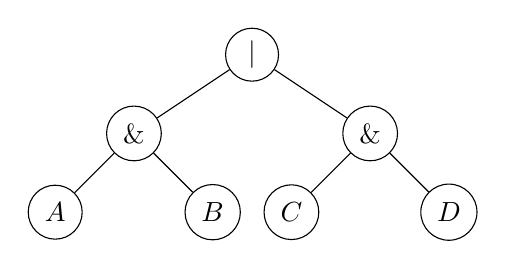
\begin{tikzpicture}[level distance=1cm,
  every node/.style={shape=circle,draw,align=center, sibling distance=3cm},
  level 1/.style={sibling distance=3cm},
  level 2/.style={sibling distance=2cm}
]
\node {$|$}
   child{node{$\&$}
     child {node{$A$} 
     }
     child {node {$B$}
     }
   } 
   child {node {$\&$}
     child {node {$C$}
     }
     child {node {$D$}
     }
   };
\end{tikzpicture}
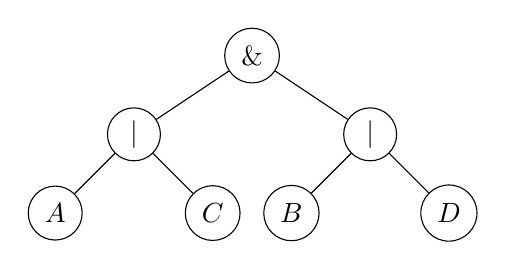
\begin{tikzpicture}[level distance=1cm,
  every node/.style={shape=circle,draw,align=center, sibling distance=3cm},
  level 1/.style={sibling distance=3cm},
  level 2/.style={sibling distance=2cm}
]
\node {$\&$}
   child{node{$|$}
     child {node{$A$} 
     }
     child {node {$C$}
     }
   } 
   child {node {$|$}
     child {node {$B$}
     }
     child {node {$D$}
     }
   };
\end{tikzpicture}
\pause

Let $t_A \oplus t_B = \max(t_A,t_B)$  and $t_A \otimes t_B = t_A + t_B$. $t_W$ cost of vector addition in codomain of $A$ and $B$  and $t_V$ cost of vector addition in codomain of $C$ and $D$
$$
t_{S1} = t_W \otimes (t_A \oplus t_B) \oplus t_V \otimes (t_C \oplus t_D) \leq (t_W \oplus t_V) \otimes ((t_A \oplus t_C) \oplus (t_B \oplus t_D)) = t_{S2} $$
with equality iff $t_A = t_B = t_C = t_D$. Showing that $S1$ is never less efficient than $S2$.
\pause
\begin{itemize} 
%\item Conjecture: For any expression constructed from $|$ $\&$, $+$, $*$ the optimal implementation is one where the total number of $\&$ and $|$ is minimal and all $\&$ and $|$ are at the top of the binary tree
% If there is any $|$ it has to appear as root of the BT
\item Replacing \lstinline$|$ by \lstinline|&| for the adjoint will not be optimal. 
% \item Is there a ``balancing'' tree algorithm?  
\end{itemize} 

\end{frame}


\begin{frame}[fragile]{Signature of the TL and AD operators}

\begin{tabular}{l|c|c|c}
  &\lstinline|void Htl(const X& x, Y& y)|  & \lstinline|Y Htl(const X& x);|& \lstinline|// Y Htl(X&& x)|\\
  &\lstinline|Htl(x,y)|  & \lstinline|auto y = Htl(x);|&  \begin{tabular}[c]{@{}c@{}} \lstinline|auto y = Htl(x);|  \\ \lstinline|//  auto y = Htl(f())| \end{tabular} \\
\Bstrut TL &
  $\begin{bmatrix} x \\ y \end{bmatrix} = \begin{bmatrix} I & 0  \\ H & 0 \end{bmatrix} \begin{bmatrix} x \\ y\end{bmatrix} $  &
  $\begin{bmatrix} x \\ y \end{bmatrix} = \begin{bmatrix} I  \\ H  \end{bmatrix} \begin{bmatrix} x \end{bmatrix} $&
  $\begin{bmatrix}y\end{bmatrix}= \begin{bmatrix}H\end{bmatrix} \begin{bmatrix}x\end{bmatrix}$
\\
\hline
\Tstrut
AD & $ \begin{bmatrix} x \\ y \end{bmatrix} = \begin{bmatrix} I & Ht  \\ 0  & 0 \end{bmatrix} \begin{bmatrix} x \\ y\end{bmatrix} $ &
$\begin{bmatrix} x \end{bmatrix} = \begin{bmatrix} I  & Ht  \end{bmatrix} \begin{bmatrix} x \\ y  \end{bmatrix} $ &
$\begin{bmatrix}x \end{bmatrix}= \begin{bmatrix}Ht\end{bmatrix} \begin{bmatrix}y\end{bmatrix}$
\\
& \lstinline|void Had(X& x, Y& y)| & \begin{tabular}[c]{@{}c@{}} \lstinline|void Had(X& x, Y&& y);|  \\ \lstinline|//X Had(Y&& y);| \\ \lstinline|//x += Had(move(y));|   \end{tabular} &\lstinline|X Had(Y&& y);|
\end{tabular}

\begin{itemize}
\item Stroustrup: return a result as a return value rather than modifying an object through an argument.
\item Option 1) In the adjoint we set $y$ to zero but memory can not be deallocated. An ``unnecessary'' addition in adjoint code for every function call\footnote{How does this overhead affect the speed of the adjoint?}
\item Option 2) still requires pass-by-reference in the adjoint
\item Option 2+3) Copy assignment needs to be \lstinline|=delete| for all objects (to avoid \lstinline|y=Htl(x)|)
\item Option 3) \lstinline|X&&| is not allowed to be a deduced type\footnote{See https://isocpp.org/blog/2012/11/universal-references-in-c11-scott-meyers}. Introduce unit-tests for this.
\end{itemize}
\end{frame}

%\begin{frame}{CppCoreGuidelines}

%   \includegraphics[width=0.9\textwidth]{param-passing-advanced.png}
%  \end{frame}



\begin{frame}[fragile]{Open issues: lvalues, prvalues, xvalues, copy/move-assignment, copy/move-constructor, copy/move elision}

  \begin{tabular}{c|c|c|c}
  Copy construction\footnote{With automatic storage duration}                      &     Copy-assignment    & Move construction & Move-assignment \\
  \begin{lstlisting}
  T a = b;

  \end{lstlisting}
    &  \lstinline|a = b;|    &   \lstinline|T a=std::move(b);|   & \lstinline|a=std::move(b);|   \\ \hline
    $\begin{bmatrix} a \\ b \end{bmatrix} = \begin{bmatrix} 1 \\ 1 \end{bmatrix} \begin{bmatrix} b \end{bmatrix}$   &
    $\begin{bmatrix} a \\ b \end{bmatrix} = \begin{bmatrix} 0 & 1 \\ 0 & 1 \end{bmatrix} \begin{bmatrix} a \\ b \end{bmatrix}$ &
    $\begin{bmatrix} a \end{bmatrix} = \begin{bmatrix} 1 \end{bmatrix} \begin{bmatrix} b \end{bmatrix}$  &
    $\begin{bmatrix} a \end{bmatrix} = \begin{bmatrix} 0  & 1 \end{bmatrix} \begin{bmatrix} a \\ b \end{bmatrix}$  \\

    \rule{0pt}{6ex}    $\begin{bmatrix} \tilde{b} \end{bmatrix} = \begin{bmatrix} 1 & 1 \end{bmatrix} \begin{bmatrix} \tilde{a} \\ \tilde{b} \end{bmatrix}$   &

       $\begin{bmatrix} \tilde{a} \\ \tilde{b} \end{bmatrix} = \begin{bmatrix} 0 & 0 \\ 1 & 1 \end{bmatrix} \begin{bmatrix} \tilde{a} \\ \tilde{b} \end{bmatrix}$ &
       $\begin{bmatrix}  \tilde{b} \end{bmatrix} = \begin{bmatrix} 1  \end{bmatrix} \begin{bmatrix} \tilde{a} \end{bmatrix}$ &
       $\begin{bmatrix} \tilde{a} \\ \tilde{b} \end{bmatrix} = \begin{bmatrix} 0 \\ 1 \end{bmatrix} \begin{bmatrix} \tilde{a} \end{bmatrix}$ \\
   \rule{0pt}{6ex}     \shortstack{\lstinline|a += b;| \\ \lstinline|b =std::move(a);|}\footnote{Note that simply \lstinline|b = a + b| would not release the resources held by \lstinline|a| at the correct time. Although the destructor would get called when \lstinline|a| goes out of scope}
    & \shortstack{\lstinline|b += a;| \\ \lstinline|a=0;|}  &  \lstinline|T b=std::move(a);| &  \lstinline|T b=a; a=0;  |

  \end{tabular}
\begin{itemize}
%  \item The adjoint of copy-construction \lstinline|T a = b;| is  \lstinline|b* = a* + b*;| \footnote{Because: $\begin{bmatrix} a \\ b \end{bmatrix} = \begin{bmatrix} 1 \\ 1 \end{bmatrix} \begin{bmatrix} b \end{bmatrix} $}

 % \item The adjoint of copy-assignment   \lstinline|a=b;| is \lstinline|b* = a* + b*; a*=0;|. \footnote{Because: $\begin{bmatrix} a \\ b \end{bmatrix} = \begin{bmatrix} 0 & 1 \\ 0 & 1 \end{bmatrix} \begin{bmatrix} a \\ b \end{bmatrix} $ then  $ \begin{bmatrix} a* \\ b* \end{bmatrix} = \begin{bmatrix} 0 & 0 \\ 1 & 1 \end{bmatrix} \begin{bmatrix} a* \\ b* \end{bmatrix}$}
 % \item The adjoint of move-construction \lstinline|T a = std::move(b);| is \lstinline|T b = std::move(a);|
 % \item The adjoint of move assignment  \lstinline|a = std::move(b);| is \lstinline|T b = std::move(a);|
 %  \item So in the adjoint code we have \lstinline|b* += a*| but \lstinline|a*| should be an rvalue.


 \item  $\begin{bmatrix} a \\ b \end{bmatrix} = \begin{bmatrix} 1 & 0 \\ 1 & 1 \end{bmatrix} \begin{bmatrix} a \\ b \end{bmatrix}$. \lstinline|b=a+b;| or \lstinline|b+=a;|. Note we have  $ \begin{bmatrix} 1 & 1 \end{bmatrix} =  \begin{bmatrix} 1 &  0 \end{bmatrix}  \begin{bmatrix} 1 & 1 \\ 0 & 1 \end{bmatrix} $.
 \item  \lstinline|void swap( T& a, T& b );| $\begin{bmatrix} a \\ b \end{bmatrix} = \begin{bmatrix} 0 & 1 \\ 1 & 0 \end{bmatrix} \begin{bmatrix} a \\ b \end{bmatrix}$
 \item Destructor \lstinline|~b;| $\begin{bmatrix} a \end{bmatrix} = \begin{bmatrix} 1 & 0 \end{bmatrix} \begin{bmatrix} a \\ b \end{bmatrix}$ adjoint \lstinline|b=0;|
\end{itemize}
\end{frame}

% \begin{frame}[fragile]{Vectors in OOPS}
%   \begin{itemize} 
%     \item We want a uniform interface to the Fortran. (Single object single responsibility). 
%    \item Vectors have several methods such as addition, scalar multiplication. 
%    \item For operators addition is an "emergent" feature that using mfla is inherited from the codomain. 
%    \item Can we view vectors as operators $\mathbb{N} \rightarrow \mathbb{R}$, i.e. interface the fortran at this level. 
%    \item Addition and scalar multiplication are now ''inherited'' from $\mathbb{R}$
%    \item Can avoid creation of temporary objects in e.g.  $x = a +  b + c$,  i.e. we will loop over the vectors a,b,c only once. With an overloaded \lstinline|operator+| that calls Fortran this is not possible.   
%   %  \item If we have an ensemble \lstinline|auto X = x1 & x2 & ... & xn| this will also introduce to possibility to eliminate all temporaries that would have to created in an expression like 
%   %    \lstinline|auto xm = X*alpha;|  where \lstinline|alpha| is a vertical concatenation of doubles. 
%    \item What is the performance penalty of these temporaries. e.g. when we compute an ensemble mean?

% \end{itemize} 
% % \begin{lstlisting} 
% %   class StateIncrement { 
% %     StateIncrement() : _val[n]  {
% %     }
% %     StateIncrement(
% %     const double& operator()(int i) const {
% %       return _val[i];       
% %     }       
% %     ~StateIncrement() { // deallocate Fortran array. RAII
% %     }
% %     double _val[n]; 
     
% %   }; 
% % \end{lstlisting} 
% % 


% \end{frame} 


\begin{frame}[fragile]{Reshaping}

There is an invertible linear transformation $G$ that maps horizontal concatenations of vectors $v_i \in V$ to vertical concatenations.


$$G: V^n \rightarrow V^n, \quad  \begin{bmatrix} v_1 & v_2 & \ldots & v_n \end{bmatrix} \mapsto  \begin{bmatrix} v_1 \\ v_2 \\ \vdots \\ v_n \end{bmatrix} $$

For clarity distinguish the domain and codomain

$$G: \Lin(\mathbb{R}^n,V) \rightarrow \Lin(\mathbb{R},V^n), \quad \begin{bmatrix}v_1 & v_2 & \ldots & v_n \end{bmatrix} \mapsto  \begin{bmatrix} v_1 \\ v_2 \\ \vdots \\ v_n \end{bmatrix} $$
\pause

For operators $A_i:  W \rightarrow V$
$$G: \Lin(W^n,V) \rightarrow \Lin(W,V^n), \quad \begin{bmatrix} A_1 & A_2 & \ldots & A_n \end{bmatrix} \mapsto  \begin{bmatrix} A_1 \\ A_2 \\ \vdots \\ A_n \end{bmatrix} $$

%Note in the current design when we have  linear operator from $A:V\rightarrow W$ we say the domain is $V$. It might be better to say that the domain is
%\begin{lstlisting}
%template<T>
%using dom = Lin<T,V>
%\end{lstlisting}

% and let vectors be derived classes from the base class \lstinline|Lin<double,V>|
\end{frame}

%\begin{frame}{Simplifying mfla}
%  \begin{itemize}
%    \item If we have a reinterpration of operator* for a Vertcat of operators do we need an implementation of Horzcat?
%    \item If we can eliminate Horzcat do we need Vertcat or is it sufficient to use the standard containers in the STL?
%   \item E.g. Given \lstinline|vector<ModelIncrement> X|. Where each element in X has operator*

%  \end{itemize}

% \end{frame}

\begin{frame}[fragile]{Iterating}
Given a linear operator $A:V \rightarrow V$. We define the nonlinear operator
\begin{align*}
  iterate(n): \Lin(V,V) &\rightarrow \Lin(V,V^n)    \\
                      A &\mapsto \begin{bmatrix} I \\ A \\ \vdots \\ A^{n-1} \end{bmatrix}
\end{align*}

\pause
Also the nonlinear operator
\begin{align*}
  normalize : V &\rightarrow V    \\
              v &\mapsto  \frac{1}{\sqrt{v^Tv}} v
\end{align*}




\end{frame}


\begin{frame}[fragile] {Naive Krylov methods}


Given a linear operator $A: V \rightarrow V$ we can construct a new linear operator


\begin{align*}
 F : V &\rightarrow \Lin(\mathbb{R}^n,V),  \\
                      v &\mapsto   \begin{bmatrix}  v & Av & A^2v & \ldots  & A^nv\end{bmatrix}
\end{align*}

then we can generate
\begin{lstlisting}
auto r = b + B*~H*Rinv*d; // b = xb-xg , d = y - H(xg)
auto A = I + B*~H*Rinv*H;
auto F = Ginv*iterate(A,n);  // or   Ginv*iterate(normalize*A,n);
auto K = F*r;
\end{lstlisting}

%%%%%%%%%%%%%%%%%%%%%%%%%%%%%%%%%%%%%%%%%%%%%%%%%%%%%%%%%%%%%%%%%%%%%%%%%%%%%%%%%%%%%%%%%%%%
%%
%% Taking the transpose is a linear operator (a tensor) similar to Ginv.
%% We could implement an operator Trans such that
%% auto xt = Trans*x
%% xt is an operator that acts on vector x so we write the inner product as
%% auto a = xt*x
%%
%% However writing
%% auto a = Trans*x*x;
%%
%% which should be equal to Trans*(x*x)
%% Wouldn't be allowed in mfla because the dom and cod of x*x wouldn't match
%%



\pause
Note that the Krylov subspace is itself a linear operator $K: \mathbb{R}^n \rightarrow V$
If we have a function object for the cost function $J: V \rightarrow \mathbb{R}$ we should be able to do composition
\begin{lstlisting}
auto JK = J * K;     // J o K: R^n --> R,  v -->  J(K*v)
\end{lstlisting}

Here $JK: \mathbb{R}^n \rightarrow  \mathbb{R}$.

Given an ensemble \lstinline|X| we should be able to do

\begin{lstlisting}
auto JKX = J * (K & X);
\end{lstlisting}

To search for the minimum of $J$ restricted to the combined Krylov and ensemble space.
%\pause

% \lstinline|Mn = iterate(M,n); dX = Mn*dx0 // M is the single time step propagator|

\end{frame}

% \begin{frame}[fragile]{Lanczos iteration}

% Let $q_j$ denote the Lanczos vectors for an operator $A$ with given $q_0$, then

% $$A q_j = \sum_{i=1}^{j+1}  q_i h_{ij}$$

% How to express this in code? e.g. Suppose we wish to solve if
% $$A x = b$$

% In the Krylov subspace with orthogonal basis $Q = \begin{bmatrix} q_1 & \cdots & q_n \end{bmatrix}$


% $$  Q^T A Q v = Q^T b $$


% We can not simply implement a function that calculates both $Q$ and $H$ because we can only return a single object. Introducing a new LanczosSystem class on which we can call getQ and getH seems not very elegant.
% Can we use template specialization for \lstinline|Prod<A,LanczosVector<A,q0,j>>| ?

% \begin{lstlisting}[basicstyle=\ttfamily\tiny]
% template<class A, class q0, int j>
% Prod<A,LanczosVector<A,q0,j> > {
%  typedef ..
%   Prod() {Aq_ = beta <A,q0,j-1> * LanczosVector<A,q0,j-1> +
%                 alpha<A,q0,j-1> * LanczosVector<A,q0,j  > +
%                 beta <A,q0,j  > * LanczosVector<A,q0,j+1>)
%                 // this should be lazy
%          }
%  codmain_type operator*(const domain_type & x) { return x*Aq_; }
%  domain_type    leval(const codomain_type & x) { ... }
%  private:
%   codomain_type Aq_;
% }
% \end{lstlisting}
% \end{frame}



\begin{frame}{Summary}
  \begin{itemize}
    \item mfla allows composition, addition, horizontal and vertical concatenation and keeps track of the adjoint for each TL.
    \item Code for e.g. block matrices (saddle point formulations), \lstinline|DualVectors|, \lstinline|Hessian| and ensembles can be generated automatically at compile time
    \item Ease of composition is essential to get flexible code.
    \pause
  \item Open issues
    \begin{itemize}
      \item Can we impose the single input, single output everywhere? 
      \item Can we exclude copy assignment (and copy construction) for all objects?
     \item how to model the relation between NL and TL/AD 
     \item How to handle linearization state of operators
     \item Automatically generate TL/AD code at compile time?
%     \item Write all C++ routines such that they are side effect free.
    \item C++11 in OOPS (use of \lstinline|auto|,  move constructors, rvalue references)
    \item Which decisions can be made at compile time to simplify the code (avoid unnecessary creation of templated code), e.g.\ the DA-formulation, the minimization algorithm, model resolution?
  \end{itemize}
  \end{itemize}
\end{frame}

% \begin{frame}[fragile]{Copy constructor, Copy assignment, Move constructors, Move assignment}
% In the current mfla we have for the L63 test model

% \begin{lstlisting}
% class L63State { 
%   L63State(const L63State & x)             = delete;  // copy ctor
%   L63State(L63State && x )                 = default; // move ctor
%   L63State& operator=(const L63State& x )  = delete;  // copy assign
%   L63State& operator=(L63State && x )      = delete;  // move assign
%   ~L63State()                              = default; // dtor
%   //etc
% };
% \end{lstlisting}

% Note in OOPS we have for L95,tstep=PT1H30M, SaddlePoint, ninner=40 nouter=2, window\_length=P1D,window\_sub=PT12H
%   \begin{itemize} 
%     \item Increment copy ctor 3802 times 
%     \item ObsAuxIncrement copy ctor 1080 times
%     \item ModelAuxIncrement copy ctor 1080 times
%     \item 
%   \end{itemize} 

% \end{frame} 

\begin{frame}[fragile]{Side effects (IO, diagnostics).  Note NL/TL/AD in a single object here} 
\begin{lstlisting} 
template<class dom>
struct Statewriter {
  typedef dom domain_type;
  typedef dom codomain_type;
  Statewriter(std::ostream & osnl,std::ostream & ostl, std::ostream &  osad) : 
                  _osnl(osnl) , _ostl(ostl), _osad(osad) { } 
  codomain_type operator()(domain_type x) const {         // 
    _osnl << x << "\n"; return x; }
  codomain_type tl(domain_type, domain_type   dx) const { // was operator*
    _ostl << dx << "\n"; return dx; }
  domain_type   ad(domain_type, codomain_type dy) const { // was leval
    _osad << dy << "\n"; return dy; }
 private: 
  std::ostream & _osnl, 
  std::ostream & _ostl,
  std::ostream & _osad; 
};
\end{lstlisting}
\pause
\begin{lstlisting} 
int main() {
//  ...
  Propagator         M( ...); 
  std::ofstream      osnl("nltraj.txt"); 
  std::stringstream  osad;     // Or /dev/null implementation 
  Statewriter<State> W(osnl, std::cout, osad);
  auto  WM  = W*M; 
  auto  WM4 = WM*WM*WM*WM; 
};
\end{lstlisting} 

\begin{itemize}
  \item Other side effects (e.g.\ canonical injections into Fortran arrays, or diagnostics) should use a similar construction.   
\end{itemize} 
\end{frame} 

\begin{frame}[fragile]{Design of objects in OOPS: Interpolate}

Current

\begin{lstlisting}
class QgFields {
// Interpolate to given location
  void interpolate  (const LocQG &, GomQG &)        const;
  void interpolateTL(const LocQG &, GomQG &)        const;
  void interpolateAD(const LocQG &, const GomQG &);
// etc
};
\end{lstlisting}
This signature suggests that $interpolate: LocQG \rightarrow GomQG$. Note AD is a non-const. 

\pause
Instead move interpolation to LocQG
$LocQg : QgField \rightarrow GomQg$
\begin{lstlisting}
class LocQG {
  void interpolate  (const Qgfields &, GomQG &)       const;
  void interpolateTL(const Qgfields &, GomQG &)       const;
  void interpolateAD(QgFields       &, const GomQG &) const;
};
\end{lstlisting}

All operators are now const member function.  Const GomQG?
\pause

Perhaps treat interpolation as a ``first class citizen''. 

\begin{lstlisting}
class Interpolate { 
  Interpolate(LocQG locQG) : _locQG(locQG)  { }
  GomQG    NL(const Qgfields &) const;
  GomQG    TL(const Qgfields &) const;
  QgFields AD(const GomQG &)    const;
};
\end{lstlisting}
\end{frame}

\begin{frame}[fragile]{Design of objects in OOPS: Derivatives and interpolation}

  $$ LocQg \colon QgField \rightarrow GomQg$$

\begin{lstlisting}
class LocQG { 
  GomQG    NL(const Qgfields &) const;  // Interpolation 
  GomQG    TL(const Qgfields &) const;  // TL of Interpolation  
  QgFields AD(const GomQG &)    const;
};
\end{lstlisting}


$$QgField\colon LocQg \rightarrow GomQg$$

\begin{lstlisting}
class QgField { 
  GomQG    NL(const LocQG &) const; // Function evaluation  
  GomQG    TL(const LocQG &) const; // The spatial derivative at a point
  LocQg    AD(const GomQG &) const; // We need linearization points here
};
\end{lstlisting}

\pause
\begin{itemize}
  \item Is this "Duality" between Functions and Domains something general?
\end{itemize}
\pause
\begin{itemize} 
  \item To handle both ``views'' should we implement $QgField \times LocQg \rightarrow GomQg$ and use currying
  \item E.g.\ if \lstinline|QgField qgfield;| and \lstinline|LocQg logqg;| ($qgfield \in QgField$  and  $logqg \in LocQg$)
  \item Then $qgfield\colon LocQg \rightarrow GomQg$ and $locqg\colon QgField \rightarrow GomQg$ 
%  \item i.e. the constructor of a GomQG take a pair LocQg QgField  
\end{itemize} 

\end{frame}

% \begin{frame}{Interpolation} 
%   Given a smooth field on the sphere  $T \in \mathcal{C}^{\infty}_{S^2, \mathbb{R}}$ and a position $r \in S^2$ we have a map 

%   $f: \mathcal{C}^{\infty}_{S^2,\mathbb{R}} \times \mathbb{R}^2 \rightarrow \mathbb{R},  (T,r) \rightarrow T(r)$ 

% The TL maps 

%   $df(T,r) = dT(T,r) + \left. \frac{\partial T}{\partial r}\right|_{(T,r)} d r$ 

% For a given $r=a$ we have

% $df(T,a) = dT(T,a)$ 

% \end{frame} 



% \begin{frame}[fragile]{Algorithms}
%   \begin{itemize}
%     \item Power iteration (Lanczos)
%     \item W and R are functors that read and write to file. (R \lstinline|domain = FileSystem|)
%     \item The structure of the algorithm is fixed at compile time.
%   \end{itemize}

%   %   \includegraphics[width=0.3\textwidth]{/home/roels/Dropbox/Linktodocuments/oops/maxplus/viz/PowerIteration2.pdf}
%    \includegraphics[width=0.3\textwidth]{\string~/Dropbox/Linktodocuments/oops/maxplus/viz/PowerIteration2.pdf}
% \end{frame}

% \begin{frame}[fragile]{Adjoint code}

% Let $\mathcal{A}_i$ be a nonlinear operator for which we recompute in the TL and AD code.

% Given $$x_3 = (\mathcal{A}_3  \circ \mathcal{A}_2 \circ \mathcal{A}_1)  (x_0)$$

% During the nonlinear integration each object $\mathcal{A}_i$ should store (and own) it's own linearization state. (No separate class for the linearization trajectory).

% This would imply that the objects $\mathcal{A}_i$ are not fully initialized after the call to the constructor. Better let \lstinline|operator()| of each object $\mathcal{A}_i$ return the TL/AD operator instead of $x_i$.\footnote{Both the highres NL and the Lowres NL should return the TL/AD of the Lowres. What about code that reads the whole Highres traj.?}


% Given $$ (A_3 \circ A_2 \circ  A_1) = (\mathcal{A}_3  \circ \mathcal{A}_2 \circ \mathcal{A}_1)  (x_0)$$



% $$\delta x_3 = (A_3 \circ A_2 \circ  A_1)*\delta x_0$$

% AD $$\delta x^*_0 = (A^T_1 \circ A^T_2 \circ A^T_3)*\delta x^*_3$$

% Each TL/AD object should be convertible to an element in the codomain such that
% we can still do composition of the nonlinear objects. i.e. in $(A_3 \circ A_2
% \circ  A_1) = (\mathcal{A}_3  \circ \mathcal{A}_2 \circ \mathcal{A}_1)  (x_0)$
% we don't compute $x_3 = \mathcal{A}_3(x_2)$ as it is not needed for the TL and
% AD only when the is an explicit request for $x_3$ e.g.\ because of composition
% with $\mathcal{A}_4$ do we calculate the value.

% \end{frame}

% \section{Semi-automatic compile time differentation}
\begin{frame}[fragile]{Composition and automatic compile time differentiation}
\begin{columns}
\begin{column}{0.3\textwidth}
\begin{lstlisting}[language=Fortran]
SUBROUTINE f(x,y)
  ! f: x -> y
  CALL h(x,z)
  CALL g(z,y)
END
\end{lstlisting}
\end{column}
\begin{column}{0.3\textwidth}
\begin{lstlisting} [language=Fortran]
SUBROUTINE ftl(x,dx,dy)
  CALL h(x,z)
  CALL htl(x,dx,dz)
  CALL gtl(z,dz,dy)
END
\end{lstlisting}
\end{column}
\begin{column}{0.3\textwidth}
\begin{lstlisting} [language=Fortran]
SUBROUTINE fad(x,dy,dx)
  CALL h(x,z)
  CALL gad(z,dy,dz)
  CALL had(x,dz,dx)
END
\end{lstlisting}
\end{column}
\end{columns}
\pause
\begin{lstlisting}
template<class G, class H>
class Prod {
 public:
  typedef typename H::domain_type   domain_type;
  typedef typename G::codomain_type codomain_type;
  Prod(const G & g,const H & h) : _g(g), _h(h) { }
  codomain_type operator()(domain_type x) const {
    return _g(_h(x));
  }
  codomain_type tl(const domain_type & x,domain_type  dx) const {
    return _g.tl(_h(x),_h.tl(x,dx));
  }
  domain_type ad(const domain_type & x,codomain_type  dy) const {
    return _h.ad(x,_g.ad(_h(x),dy));
  }
 private:
  const G _g;
  const H _h;
};
\end{lstlisting}
\pause
\begin{itemize}
\item Not optimal for $k \circ f = k \circ (g \circ h)$ but $(k \circ g) \circ h$ is fine if $h$ is "elementary".
\item With addition: $k \circ (g + h)$ is fine but  $k \circ (g + h \circ p)$ is not optimal
\end{itemize}


\end{frame}

\begin{frame}[fragile]{Composition and automatic compile time differentiation}
\begin{lstlisting}
template<class G, class H>
class Prod {
 public:
  typedef typename H::domain_type   domain_type;
  typedef typename G::domain_type   Gdomain_type;
  typedef typename G::codomain_type codomain_type;
  Prod(const G & g,const H & h) : _g(g), _h(h), _x(0), _y(0) { }
  codomain_type operator()(domain_type x) const {
    _x = x;
    _y = _h(x); 
    return _g(_y);
  }
  codomain_type tl(domain_type dx) const {
    return _g.tl(_y,_h.tl(_x,dx));
  }
  domain_type ad(codomain_type dy) const {
    return _h.ad(_x,_g.ad(_y,dy));
  }
 private:
  domain_type  _x; 
  Gdomain_type _y; 
  const G _g;
  const H _h;
};
\end{lstlisting}


Here \lstinline|_x| and \lstinline|_y| only get initialized after the call to \lstinline|operator()|  

\end{frame}

\begin{frame}[fragile]{}

\begin{lstlisting}
template<class G, class H>
class Composition {
 public:
  typedef typename H::domain_type   domain_type;
  typedef typename G::codomain_type codomain_type;
  Composition(const G & g,const H & h) : _g(g), _h(h) { }
  auto operator()(domain_type x) const {
    return g(h(x));
  }
  auto derivative(domain_type x) const {
    return TL<G>(_g,_h(x))*TL<H>(_h,x);
  }
 private:
  const G _g;
  const H _h;
};
\end{lstlisting}




\end{frame} 


% \begin{frame}[fragile]{Composition and automatic compile time differentiation. Better?}
% \begin{columns}
% \begin{column}{0.33\textwidth}
%   \begin{lstlisting}[language=Fortran]
% SUBROUTINE f(x,y)
%   ! f: x -> y
%   CALL h(x,z)
%   CALL g(z,y)
% END
% \end{lstlisting}
% \end{column}
% \begin{column}{0.33\textwidth}
%   \begin{lstlisting} [language=Fortran]
% SUBROUTINE ftl(x,dx,y,dy)
%   CALL htl(x,dx,z,dz)
%   CALL gtl(z,dz,y,dy)
% END
% \end{lstlisting}
% \end{column}
% \begin{column}{0.33\textwidth}
%   \begin{lstlisting} [language=Fortran]
% SUBROUTINE fad(x,dy,y,dx)
%   CALL gad(h,x, dy,dz)
%   CALL had(x,dx,)
% END
% \end{lstlisting}
% \end{column}
% \end{columns}

% \begin{lstlisting}
% template<class G, class H>
% class Prod {
%  public:
%   typedef typename H::domain_type   domain_type;
%   typedef typename G::codomain_type codomain_type;
%   Prod(const G & g,const H & h) : _g(g), _h(h) { }
%   codomain_type operator()(domain_type x) const {
%     return _g(_h(x));
%   }
%   std::pair<codomain_type, codomain_type> tl(std::pair<domain_type, domain_type>  dx) const {
%     return _g.tl(_h.tl(dx));
%   }
%   std::pair<domain_type,domain_type> ad(std::pair<domain_type, codomain_type> dy) const {
%     return _h.ad(_g.ad(dy));
%   }
%  private:
%   const G _g;
%   const H _h;
% };
% \end{lstlisting}

% \begin{itemize}
%   \item Here \lstinline|std::pair<domain_type, domain_type> dx| is an element in the tangent bundle TM. Elements of TM contain base points $x$ and tangent vectors $dx$.
%   \item \lstinline|std::pair<domain_type, codomain_type> dy| is an element of cotangent bundle?
%   \item Should we introduce the pullback  $h_* g =  g \circ h$ to do composition?
% \end{itemize}
% \end{frame}

% \section{L63 Example}

% \begin{frame}[fragile]{L63 Example}
% \begin{lstlisting}
% struct L63 {
%   L63(double sigma, double rho, double beta) :
%       _sigma(sigma),  _rho(rho), _beta(beta) {}
 
%   typedef L63State domain_type;
%   typedef L63State codomain_type;

%   L63State operator()(L63State x)  const {
%     return {_sigma*(x[1] - x[0]),
%          x[0]*(_rho-x[2]) - x[1],
%           x[0]*x[1] - _beta*x[2]};
%   }

%   L63State tl(L63State x, L63State dx) const {
%     return {-_sigma*dx[0] +      _sigma*dx[1]              ,
%         (_rho-x[2])*dx[0] -             dx[1] -  x[0]*dx[2],
%                x[1]*dx[0] +        x[0]*dx[1] - _beta*dx[2]};  
%   }

%   L63State ad(L63State x, L63State dx) const {
%     return {-_sigma*dx[0] + (_rho-x[2])*dx[1] +  x[1]*dx[2],
%              _sigma*dx[0] -             dx[1] +  x[0]*dx[2],
%                           -        x[0]*dx[1] - _beta*dx[2]};
%   }   
%  private: 
%   double  _sigma, _rho, _beta;
% };
% \end{lstlisting} 
% \end{frame}

% \begin{frame}[fragile]{RK4}
% \begin{lstlisting}
% template<class HF> 
% struct RK4 {
%   RK4(HF hf) : _hf(hf) {}    
%   template<class T> 
%   T operator(T x) {
%     T hk1 = hf(x);
%     T hk2 = hf(x + 1/2*hk1);
%     T hk3 = hf(x + 1/2*hk2);
%     T hk4 = hf(x +     hk3);
%     return x + 1/6*(hk1 + 2*hk2 + 2*hk3 + hk4);
%  }
%  private: 
%    HF _hf;
% };
%  \end{lstlisting}

% % \begin{itemize}
% %   \item  Note $\begin{bmatrix} I \\ hf \end{bmatrix} x $ can take argument by rvalue reference.
% % \end{itemize}
% % $ \begin{bmatrix} x \\ hk1 \\ t \end{bmatrix}  = \begin{bmatrix} I & 0 \\ 0 & I \\ I & \frac{1}{2} \end{bmatrix} \begin{bmatrix} x \\ hk1\end{bmatrix}  $ \hspace{1cm}
% % $ \begin{bmatrix} x \\ hk1 \\ hk2 \end{bmatrix}  = \begin{bmatrix} I & 0 & 0 \\ 0 & I & 0 \\ 0 & 0 & hf'  \end{bmatrix} \begin{bmatrix} x \\ hk1 \\ t \end{bmatrix}  $

% % $$ z = \begin{bmatrix} 1 & 1/6 \end{bmatrix} \begin{bmatrix} 1 & 0 & 0  & 0 & 0 \\ 0 & 1 & 2 & 2 & 1 \end{bmatrix}    \begin{bmatrix} x \\ hk1 \\ hk2\\ hk3 \\ hk4\end{bmatrix}$$
% \end{frame}

% \begin{frame}[fragile]{RK2}
% \begin{lstlisting}
% template<class F>
% struct RK2 {
%   RK2(const F f,double h) : _f(f), _h(h) {}
%   template<class T> // if T is
%   auto operator()(T x) {
%     auto k1 = _h*_f(x);
%     auto k2 = _h*_f(x+k1/2);
%     return x+k2;
%   }
%   private:
%   F _f; double _h;
%  };
% \end{lstlisting}


% 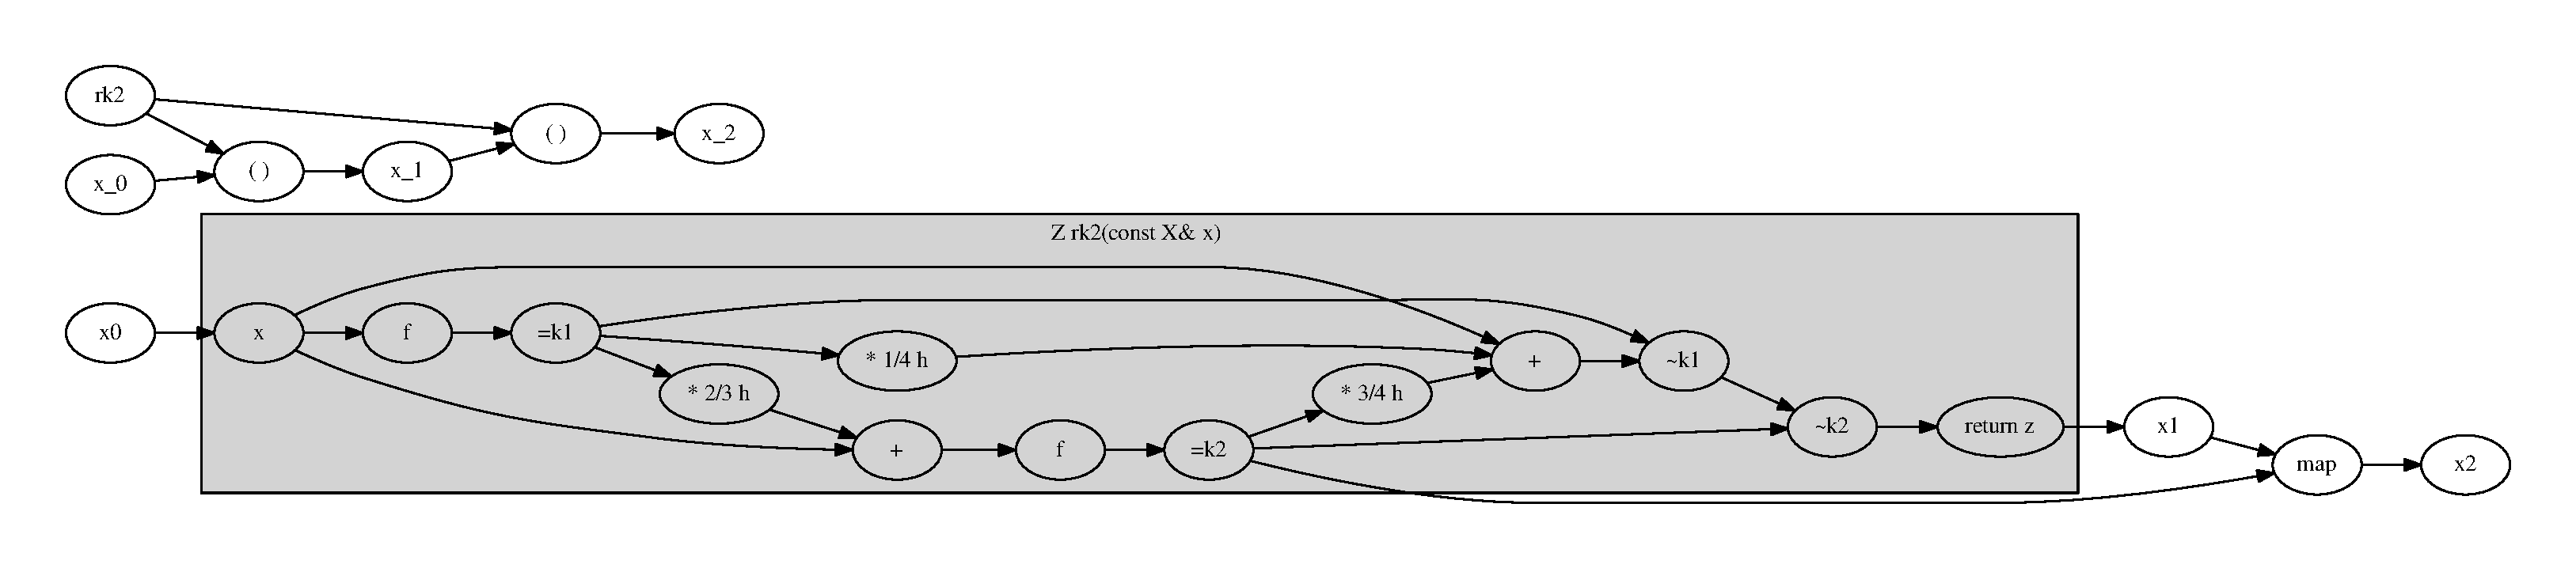
\includegraphics[width=\textwidth]{rk4a.pdf}

% \begin{itemize}
%   \item Memory layout of recomputed values k1 k2 versus stored values x0 x1?
%   \item Reverse x0 x1 stack before adjoint computation to reduce cach missesn?
% \end{itemize}
% \end{frame}

% \begin{frame}[fragile]{RK2}
% \begin{lstlisting}
% template<class HF>
% struct RK2 {
%   RK2(HF hf) : hf(hf) {}
%   T operator()(T x) {
%     return x + hf(x + hf(x)/2);
%   }
%  private:
%   HF hf;
% };
% \end{lstlisting}

% \begin{lstlisting}
%   RK2 M(hf);
%   auto z = M(x);
% \end{lstlisting}

% $ z  = \begin{bmatrix} 1 & 0 &  hf \end{bmatrix} \begin{bmatrix} I & 0 \\ 0 & I \\ I & \frac{1}{2} \end{bmatrix}\begin{bmatrix} I \\ hf \end{bmatrix} x $
% \end{frame}

% \begin{frame}[fragile]{Higher order derivative}
%   \begin{lstlisting}
%    auto D(Sin s)   {return Cos();}
%    auto D(Cos c)   {return -1*Sin();}
%    auto D(Obsop h) {return h; } //???

%    templat<class F,class G>
%    auto D(Sum<F,G> s) {return D(s._expr1) + D(s._expr2);}

%    templat<class F,class G> // Chain rule
%    auto D(Comp<F,G> p) {return comp(D(p._expr1),p._expr2)*D(p._expr2));}

%    templat<class F,class G> // Product rule
%    auto D(Prod<F,G> p) {return D(p._expr1)*p._expr2 + p._expr1*D(p._expr2);}

%   \end{lstlisting}


% \end{frame}

% \begin{frame}



% \begin{frame}[fragile]{Class design for nonlinear operators}
% \begin{lstlisting}

% class myop {
%  public:
%   myop(xmlconfig) { };
%   typedef xxx dom;
%   typedef yyy cod;
%   struct NL {cod operator()(dom&& x ){_x(x); x*x; return y; } };
%   struct TL {cod operator* (dom&& dx){return 2*_x*dx} };
%   struct AD {dom operator* (cod&& dy){     ...; return dx;} };
%   NL nl;
%   TL tl;
%   AD ad;
%  private:
%   dom _x;
% };
% \end{lstlisting}

%\begin{lstlisting}
%template<typename cod, typename T, typename dom>
%class Prod : public mapping<cod,dom> {
%  Prod(mapping<cod,T> e1, mapping<T,dom> e2) {}
%};
% \end{lstlisting}
% \begin{itemize}
%   \item No need for \lstinline|operator~| to take transpose. We have access to \lstinline|myop::ad|
%   \item Note domain of TL should be the tangent space at \lstinline|_x|
% \end{itemize}
% \end{frame}


%----------------------------------------------------------------------%
%                    Unit tests                                        %
%----------------------------------------------------------------------%

% \section{Unit tests}

% \begin{frame}{Unit tests}
% \begin{itemize}
%    \item Two obvious candidates for unit test in the IFS are the TL and the AD test.
%    \item We can't do unit tests on subroutines. \begin{itemize}
%        \item E.g.\ a unit test that tests whether larchetl is the tl of larche for a specific choice of logicals is not sufficient. It does not tell us anything about proper functioning (have setup routines been called correctly etc.) of 4D-VAR code.
%      \end{itemize}
%        \item NL/TL/AD shoud be objects. That are valid (i.e. properly initialized) NL/TL and TL/AD object for any possible choice of logicals.
%     \item The unit tests should try to falsify the hypothesis that the object is valid. With the current IFS structure this is not possible for the Fortran code.
%   \end{itemize}


% \end{frame}


%-----------------------------------------------------------------------%
%   Singular vectors
%-----------------------------------------------------------------------%
% \section{Refactoring singular vector calculation}
% % Q: If the Lanczos/CG algorithm can be represented as a DAG can we compute e.g. sensitivity of the leading singular value w.r.t. "external inputs" by one adjoint integration?
% % \begin{frame}{opk.F90}
% %   \begin{itemize}
% %     \item OPK/IFS CALLs to CAININ (45/89)  and CAIN (32/78)
% %     \item a
% %   \end{itemize}
% % \end{frame}


% \begin{frame}[fragile]{C++ SVs}
% \begin{lstlisting}
% CAININ   C2F;  // Identity operator. Send C control variable to SPA3.
% CAIN     F2C;  // Send C Control variable to Fortan SPA3

% //     - if NEWNORMT0=1 norm=total energy with q-term
% //     - if NEWNORMT0=2 norm=kinetic energy
% //    - if NEWNORMT0=3 norm=squared vorticity
% //     - if NEWNORMT0=4 norm=squared stream-function
% //     - if NEWNORMT0=5 norm=rotational kinetic energy
% CHNORM<NEWNORMTO> CN0;

% // spectral truncation alternative SPTRLCZ<nwtrmin0,nwtrmax0> S0;
% SPTRLCZ  S0(nwtrmin0,nwtrmax0);
% SPTRLCZ  S1(nwtrmin1,nwtrmax1);

% // non linear integration (C2F and F2C are part of L)
% CNT3NL  L('BK0000000');

% // Grid point localization (Perhaps better take NW,SE points  with type Location)
% LCNORTL<LOCNORM> T(ALAT1, ALAT3, ALON1,ALAT3, NLEVMIN,NLEVMAX);

% S1TLS0CN0 = S1*T*L*S0*CN0;

% OPK       = ~S1TLS0CN0*S1TLS0CN0;

% \end{lstlisting}

%// Linearize NLF arond forecast from x0
%NLFx0  = NLF(x0);

%SVs = svd<10>(NLFx,dx0)


% \end{frame}



% \begin{frame}[fragile]{NL/TL/AD class design and unit testing}
% \begin{lstlisting}

% template<class T>
% struct NL {
%   typedef typename T::domain_type    domain_type;
%   typedef typename T::codomain_type  codomain_type;
%   NL(T t) : _t(t) {}
%   TL<T> operator(domain_type && x)  {
%     return TL<T>(x);
%   } // change to perfect forwarding
%  private:
%   T _t;
% }


% template<typename cod,typename dom>
% Myop : public mapping<cod,dom>  {
%   struct NL {cod operator()(dom&& x ){_x(x); ...; return y; } };
%   struct TLAD {cod operator* (dom&& dx){       ...; return dy;} };
%   struct {dom operator* (cod&& dy){       ...; return dx;} };
%   NL nl; TL tl; AD ad;
%  private:
%   dom _x;
% } ;

% \end{lstlisting}

% \end{frame}





% \begin{frame}[fragile]{Partial template specialization (skip this)}

% Implement
% \begin{lstlisting}
% class Sum<ModelIncrement,ModelIncrement> {
%   Sum(const ModelIncrement& x1,const ModelIncrement& x2) {...}
%   operator ModelIncrement() const { // Conversion operator
%     //Do the addition (call Fortran)
%   }
% };
% \end{lstlisting}

% And remove \lstinline|operator+| from the ModelIncrement class. ModelIncrement addition is now lazy. Only when we e.g. assign to an object of type ModelIncrement do we perform calculations.
% A \lstinline|Sum<Sum<Increment,ModelIncrement>,ModelIncrement>>| is now possible because \lstinline|Sum<Increment,ModelIncrement>| is convertible to ModelIncrement, i.e. no need for template specializations for \lstinline|Sum<Sum<Sum<T,T>,T>,T>|


% Better? implement an overloaded operator+ in class Vertcat (all classes in mfla) which takes an arbitrary type T as argument, the typedef constructions will ensure that the domains and codomains match, i.e. no need to introduce  a base class \lstinline|Lin<dom,cod>| from which all operators inherit.

% \pause
% If we choose a single representation for each object what is the best way to achieve this?
% \begin{lstlisting}
% template<class T1,class T2>
% class Transpose<Sum<T1,T2>> : public Sum<Transpose<T1>, Transpose<T2>> {
%   Transpose(const Sum<T1,T2>& s) :  Sum(~s.e1,~s.e2) { }
% }
% \end{lstlisting}

% Or

% \begin{lstlisting}
% template<class T1,class T2>
% Sum<Transpose<T1>,Transpose<T2> operator~(const Sum<T1,T2>& e) {
%    return Sum(~s.e1,~s.e2); }
% \end{lstlisting}


% %Public inheritance models an ``is-a'' relation. Read as the Transpose of the sum of T1 and T2 is-a Sum of the transpose of T1 and the transpose of T2.
% %Although inheritance models a perfect is-a relations here it is probably better avoided.
% % Better to model this at the creator function level? Note there is no partial template specialization for functions need overloading here. Do we get the recursion?
% \end{frame}

%--------------------------------%
%
%--------------------------------%

% \section{States and Geometry}

% \begin{frame}[fragile]{States}
% If we have a basis for our vector space than  any vector can be written as a linear combination

% $$\vec{x} = \sum_i a_i \vec{e}_i$$

% And if the basis is clear from context we often identify the vector with the coefficients which is written as a column vector. Should we instead keep the basis in the definition of $\vec{x}$.
% Is this what the geometry class in OOPS should be?


% \begin{lstlisting}
% Sphericalharmonics<1279,137> B; // Sphericalharmonics B(1279,137)
% \end{lstlisting}

% There is a template specialization for the Laplacian that can act on spherical harmonics


% \begin{lstlisting}
%   auto x    = B*a;
%   auto Lapx = Lap*x;
% \end{lstlisting}

% Note we should actually write these expression for fields seperately so a state is

% \pause

% \begin{lstlisting}
% auto x = B*(T & p  & div & vor & q) ;
% auto x = Bsh*(T & p & div & vor ) & Bgr*q;
% \end{lstlisting}

% \pause
% No seperate State class in OOPS.
% \begin{itemize}
%   \item Interpolation is a property of the spherical harmonics or the finite elements.
%   \item \lstinline|x = FFT(T & p  & div & vor & q); // automatically parallel over fields|
%   \item Does it make sense to have vertical concatentation of fields with different units?
% \end{itemize}

% \end{frame}



% \begin{frame}[fragile]{FFT}

% \begin{lstlisting}
% template<class cod,class dom>
% class FFT {
%  public:
%   typedef domain_type    cod
%   typedef codomain_type  dom
%   FFT()    {
%     int N = dom::size();
%     // In theory the optimal plan could be determined at compile time?
%     fftw_complex *in, *out;
%     in = (fftw_complex*) fftw_malloc(sizeof(fftw_complex) * N);
%     out = (fftw_complex*) fftw_malloc(sizeof(fftw_complex) * N);
%     int sign = 1 // or -1;
%     unsigned flags = FFT_MEASURE ;  //FFT_PATIENT
%     _plan = fftw_plan fftw_plan_dft_1d(n, in, out, sign,flags); // LON
%     // _plan = fftw_plan fftw_plan_dft_2d(n0, n1, in, out, sign,flags); // LON
%   }

%   cod operator*(dom&& x) {
%     in = &x;
%     fftw_execute(_plan) ;
%     return *out;
%   }
%   ~FFT() {
%     fftw_destroy_plan(_plan);
%     fftw_free(in); fftw_free(out);
%   }
%  private:
%   fftw_plan _plan;
% }
% \end{lstlisting}

% \end{frame}

%\begin{frame}[fragile]{Perfect forwarding in C++11}
%
%\begin{lstlisting}
%// Creator function
%template<class ExprT>
%Transpose<ExprT> operator~(const ExprT& e) {
%  return Transpose<ExprT>(e);
%}
%\end{lstlisting}
%
%In  C++11 change to
%
%\begin{lstlisting}
%/// Creator function
%template<class ExprT>
%Transpose<ExprT> operator~(ExprT&& e) {
%  return Transpose<ExprT>(std::forward<ExprT>(e));
%}
%\end{lstlisting}
%
%In the context given above \lstinline|ExprT&&| is a universal reference\footnote{https://isocpp.org/blog/2012/11/universal-references-in-c11-scott-meyers}
%
%Reference collapsing rules
%\begin{itemize}
%  \item \lstinline|A& &| becomes \lstinline|A&|
%  \item \lstinline|A& &&|  becomes \lstinline|A&|
% \item  \lstinline|A&& &| becomes \lstinline|A&|
% \item \lstinline|A&& &&| becomes \lstinline|A&&|
%\end{itemize}
%
%\begin{itemize}
%  \item when \lstinline|operator~| is called with an lvalue of type A for ExprT1 then ExprT1 resolves to \lstinline|A&| and therefore the type becomes \lstinline|A&| by the reference collapsing rules.
%  \item When called with an rvalue the argument type becomes \lstinline|A&&|
%\end{itemize}
%
%\end{frame}





%\begin{frame}[fragile]{Coupled Data assimilation (and DA for Limited area models) }
%How to handle boundary conditions in limited area DA?



%\end{frame}


%\begin{frame}{Addition, vertical and horizontal concatenation of nonlinear operator}
%  Given two nonlinear operators
%  The spherical harmonics know how to do interpolation.
%  $$f:\mathrm{dom}(f) \rightarrow \mathrm{cod}(f),  x \mapsto f(x)$$ and
%  $$g: \mathrm{dom}(g) \rightarrow \mathrm{cod}(g), y \mapsto g(y)$$  we can define:
%
%  \begin{itemize}
%    \item $f \times g :\mathrm{dom}(f) \times\mathrm{dom}(g)   \rightarrow \mathrm{cod}(f) \times \mathrm{cod}(g) , (x,y) \mapsto (f(x), g(y)) $. BlockDiag(f,g)
%    \item $f \circ g : D_g \rightarrow  C_f, y \mapsto f(g(y))$ matrix multiplication. Requires $D_f=C_g$.
%    \item $f | g : \mathrm{dom}(f) \rightarrow  C_f \times C_g , x \mapsto (f(x), g(x))$ Vertical concatentation. Requires $D_f = D_g$
%    \item $f \& g: \mathrm{dom}(f) \times  D_g \rightarrow  C, (x,y) \mapsto f(x) + g(y) $.  Horzcat. Requires $C_f = C_g$
%  \item $f + g: \mathrm{dom}(f) \rightarrow \mathrm{cod}(f), x \mapsto f(x) + g(x)$ Matrix addition. Requires addition in $C$
%
%    \item $\alpha f$  left Scalar multiplication: If $C_f$ has scalar multiply.
%    \item $f \alpha$  Right scalar multiplication if $D_f$ has scalar multiply.  ?
%  \end{itemize}
%
%
%\end{frame}
%
%
%\begin{frame}[fragile]{Lambda expressions (transpose?)}
%  \begin{lstlisting}
%#include<tuple>
%#include<iostream>
%#include <functional>
%using namespace std
%
%template<class cod,class dum, class dom>
%function<cod(dom)> operator*(function<cod(dum)> g, function<dum(dom)> f) {
%  return [f,g](const dom & x) {return g(f(x));}; }
%
%template<class cod, class dom>
%function<cod(dom)> operator*(double a,function<cod(dom)> f) {
%   return [f,a](const dom & x) {return a*f(x);}; }
%
%//template<class cod, class dom>
%//function<cod(dom)> operator*(function<cod(dom)> f,double a) {
%//   return [f,a](const dom & x) {return f(a*x);}; }
%
%template<class cod, class dom>
%function<cod(dom)> operator+(function<cod(dom)> g,function<cod(dom)> f) {
%  return [f,g](const dom & x) {return g(x) + f(x);}; }
%
%template<class cod1,class cod2,class dom>
%function<std::tuple<cod1,cod2>(dom)> operator|(function<cod1(dom)> f, function<cod2(dom)> g) {
%  return [f,g](const dom & x) {return make_tuple(f(x),g(x));}; }
%
%template<class cod,class dom1,class dom2>
%function<cod(tuple<dom1,dom2>)> operator&(function<cod(dom1)> f,function<cod(dom2)> g) {
%  return [f,g](const tuple<dom1,dom2> & x) {return f(get<0>(x)) + g(get<1>(x));}; }
%\end{lstlisting}
%\end{frame}
%

% \begin{frame}[fragile]{Behavorial specification of mfla}
% \begin{enumerate}
%   \item $A \circ A^{-1}  = I$
%   \item $\begin{bmatrix}A & B \end{bmatrix} \circ \begin{bmatrix} C \\ D \end{bmatrix} = A \circ C + B \circ D$
%   \item $\begin{bmatrix}A & A \end{bmatrix} \circ \begin{bmatrix} C \\ D \end{bmatrix} \mapsto
%  A \circ \begin{bmatrix} I & I \end{bmatrix}  \circ \begin{bmatrix} C \\ D \end{bmatrix} \mapsto A \circ (C + D) $
%   \item $A   \begin{bmatrix} v_1 & v_2 \end{bmatrix} = \begin{bmatrix} Av_1 & A v_2 \end{bmatrix}$ For $v_i$ vectors but not for operators.
%  %  \item $ \begin{bmatrix} v  & B \end{bmatrix}  =  \begin{bmatrix} A v & A B \end{bmatrix}$? In RPCG
% \end{enumerate}

% \end{frame}

% \begin{frame}{Combining calculus with linear algebra}

% Given a map $\phi: M \rightarrow N$ the derivative $d \phi$ is map between tangent bundles\footnote{$TM = \mathop{\bigcup}_{x\in M} \{ (x,y) | y \in T_x M$\}}

% \begin{align*}
%   d \phi: TM   &\rightarrow TN  \\
%   (x, \delta x) &\mapsto (\phi(x),d\phi_x \delta x)
% \end{align*}

%  The derivative at a point (the differential at $x$) is

%  $$d \phi_x: T_x M   \rightarrow T_{\phi(x)} N$$


% % \includegraphics[width=0.333\textwidth]{330pxPushforward.png}

% \end{frame}


% \begin{frame}{Combining calculus with linear algebra}

% Given a map $\phi: M \rightarrow N$ the derivative $d \phi$ is map between tangent bundles\footnote{$TM = \mathop{\bigcup}_{x\in M} \{ (x,y) | y \in T_x M$\}}

%  $$d \phi: TM   \rightarrow TN$$

%  The derivative at a point (the differential at $x$) is

%  $$d \phi(x): T_x M   \rightarrow T_{\phi(x)} N$$

% Composition with  $\psi: N \rightarrow P$ gives

% $$\psi \circ \phi : M \rightarrow P, x \mapsto  \psi(\phi(x))$$

% $$d (\psi \circ \phi) : TM \rightarrow TP, \quad (x,\delta  x) \mapsto  d\psi(d\phi(x,\delta x)) $$

% If we take the derivative at a point

% $$d (\psi \circ \phi)_x : T_x M \rightarrow T_{\psi(\phi(x))}P, \quad \delta x \mapsto  d\psi_{\phi(x)}  * d\phi_x  * \delta x)) $$

% \end{frame}




% \begin{frame}[fragile]
% \begin{tikzpicture}
%   \node (M) {$M$};
%   \node[right=6cm of M] (N) {$N$};
%   \node[above=3cm of M] (TM) {$T_xM$};
%   \node[above=3cm of N] (TN) {$T_{\phi(x)} N$};
%   \draw[very thick, ->]
%    (M) edge node[fill=white] (phi) {$\phi$} (N)
%    (TM)  edge node[fill=white] (jac)  {$\D\phi_x$} (TN)
%    (M)   edge node[fill=white] (Dphi) {$\D\phi$} (jac)
%    (phi) edge node[fill=white] (ss)   {$\D$ }      (Dphi)
%    (TN)  edge[bend right=40]  node[fill=white] (Dhixt) {$\D\phi^T_x$} (TM)
%    (jac) edge node[fill=white] (trans) {$T$} (Dhixt);
%  \end{tikzpicture}

% \begin{tikzpicture}
%   \node (M) {$M$};
%   \node[right=6cm of M] (N) {$N$};
%   \node[above=3cm of M] (TM) {$T_xM$};
%   \node[above=3cm of N] (TN) {$T_{\phi(x)} N$};
%   \draw[very thick, ->]
%    (M) edge node[fill=white] (phi) {$\phi$} (N)
%    (TM)  edge node[fill=white] (jac)  {$\D\phi_x$} (TN)
%    (M)   edge node[fill=white] (Dphi) {$\D\phi$} (jac)
%    (phi) edge node[fill=white] (ss)   {$\D$ }      (Dphi)
%    (TN)  edge[bend right=40]  node[fill=white] (Dhixt) {$\D\phi^T_x$} (TM)
%    (jac) edge node[fill=white] (trans) {$T$} (Dhixt);
%  \end{tikzpicture}




% \end{frame}



% \begin{frame}[fragile]{Design of objects in OOPS: Step}
% \begin{lstlisting}
% class IncrementL95 : public oops::GeneralizedDepartures , .. {
%   void stepTL(const TLML95 &, const ModelBiasCorrection &);
%   void stepAD(const TLML95 &, ModelBiasCorrection &);
% \end{lstlisting}

% Non-const TL and AD.

% \begin{lstlisting}
% void IncrementL95::stepTL(const TLML95 & tlm, const ModelBiasCorrection & bias) {
%   tlm.stepTL(fld_, time_, bias);
% }
% \end{lstlisting}

% And we then have

% \begin{lstlisting}
% void TLML95::stepTL(FieldL95 & xx, util::DateTime & vt,
%                     const ModelBiasCorrection & bias) const {
% //etc
% const ModelTrajectory * traj = this->getTrajectory(vt);
% // etc
% }

% void TLML95::stepAD(FieldL95 & xx, util::DateTime & vt,
%          ModelBiasCorrection & bias) const {
% // etc
% }
% \end{lstlisting}

% Better avoid DateTime here
% \lstinline|FieldL95 TLML95::stepTL(const FieldL95 & xx, const ModelBiasCorrection & bias) const { } |

% \end{frame}

% \begin{frame}[fragile]{Folds, map, reduce, scans}

% A list is \lstinline|x1:x2:x3:[]|. Normally written in code as \lstinline|[x1,x2,x3]|

% %  \includegraphics[width=0.49\textwidth]{foldl.png}
% %  \includegraphics[width=0.49\textwidth]{foldr.png}

%   \begin{lstlisting}

% concat  = foldr (:)
% sum     = foldr (+) 0
% product = foldr (*) 1
% compose = foldr (.) id

% \end{lstlisting}

% scanr and scanl are similar but produce a list with the intermediate results

% \lstinline|Linv = scanl (M +) x0 | acting on a list \lstinline|[q]| of model errors produces a list \lstinline|[x]| of states.


% \end{frame}

% \begin{frame}{Automatic code generation for the Fortran interface?}

%   If all operators in OOPS follow this functor like object structure with NL, TL and AD code
%   Can we unify the interface to the Fortran routines and generate the code automatically?



%   For unit testing it would help if all operators follow the same interface to automatically test the TL is linear version of NL and the AD is the adjoint of TL. But also ensure the copy-construction has been disabled, that move assignment is enabled, etc.
% \end{frame}

% \begin{frame}{Pure Fortran routines}
% \begin{itemize}

%   \item Can we make all Fortran routines side effect free\footnote{A side effect is a result of an operator, expression, statement, or function that persists even after the operator, expression, statement, or function has finished being evaluated.
% }, i.e. pure (elemental) routines? In particular no IO, no persistent memory allocation
% \end{itemize}
% \end{frame}

% \begin{frame}{Observation independent model}
%   \begin{itemize}
%     \item Currently the obs operator is being refactored such that it will be independent of the model.
%     \item Can we also make the model independent of the observation operator?
%     \item What decision can be made at compile time, e.g.\ the choice of minimizer.
%   \end{itemize}
% \end{frame}



%\begin{frame}{Addition of increments to states}

%In many papers we write $\vec{x}^a = \vec{x}^b + \vec{\delta x}$
%What does this equation mean in a thermodynamic system?

% \end{frame}

\begin{frame}[fragile]{Restructuring the Hessian}  

\begin{equation}
\left\| 
\begin{bmatrix} 
 \opl{I}   &         &                 &     \\
 -\opl{M}_1 & \opl{I} &                &     \\
            &  \ddots & \ddots         &      \\
            &         & -\opl{M}_{N-1} & \opl{I} \\ \hline
  \opl{H}_0 &         &                 &         \\              
            &  \opl{H}_1     &          &         \\
            &                & \ddots   &        \\ 
            &                &          & \opl{H}_{N-1}   
\end{bmatrix} 
\begin{bmatrix}
 \delta x_0 \\
 \delta x_1 \\ 
 \vdots  \\
 \delta x_{N-1} 
\end{bmatrix}
- 
\begin{bmatrix} 
b_0 \\
b_1 \\ 
\vdots \\
b_{N-1} \\ \hline
d_0 \\
d_1 \\
\vdots \\
d_{N-1}
\end{bmatrix} \right\|_{\mathrm{diag}(D^{-1},R^{-1})} 
\end{equation}

Reordering the rows gives 

\begin{equation}
\left\| 
\begin{bmatrix} 
  \opl{I}   &                &                 &     \\
  \opl{H}_0 &                &                 &         \\              
 -\opl{M}_1 & \opl{I}        &                &     \\
            &  \opl{H}_1     &                &         \\
            &  -\opl{M}_2    & \opl{I}        &     \\
            &                &  \opl{H}_2      &         \\
            &                &  \ddots & \ddots         &      \\
            &                &                & -\opl{M}_{N-1} & \opl{I} \\ 
            &                &                &          & \opl{H}_{N-1}   
\end{bmatrix} 
\begin{bmatrix}
 \delta x_0 \\
 \delta x_1 \\ 
 \vdots  \\
 \delta x_{N-1} 
\end{bmatrix}
- 
\begin{bmatrix} 
b_0 \\
d_0 \\
b_1 \\ 
d_1 \\
\vdots \\
b_{N-1} \\ 
d_{N-1}
\end{bmatrix} 
\right\|_{X2}
\end{equation}

\end{frame} 




\section{GOM+ control variable (flexibility of the OOPS code)}
\begin{frame}{GOM+-arrays as control variable. Interpolation as a strong constraint}
The weak constraint 4D-VAR cost function can be written as (4D-vector notation)

$$  J(\vec{x}) =  \frac{1}{2}\|\mathcal{H}(\mathcal{V}(\vec{x}))-\vec{y}\|^2_{\op{R}^{-1}} +  \frac{1}{2}\|\mathcal{L}(\vec{x}) - \vec{p}^b\|^2_{\op{D}^{-1}}  = \tilde{J}_o(\vec{x}) + J_q(\vec{x})$$

Here $\mathcal{V}(\vec{x})$ is the mapping from 4D model states to 4D-GOM+-arrays.
\pause
$$J(\vec{x},\vec{z}) =  \frac{1}{2}\|\mathcal{H}(\vec{z})-\vec{y}\|^2_{\op{R}^{-1}} +  \frac{1}{2}\|\mathcal{L}(\vec{x}) - \vec{p}^b\|^2_{\op{D}^{-1}} = J_o(z) + J_q(x)$$

subject to  $\mathcal{V}(\vec{x}) - \vec{z} = \vec{0}$.


\pause

Incremental formulation with GOM+-arrays as control variable
\begin{equation}
  \left( \op{I} + \op{V} \op{L}^{-1} \op{D} \op{L}^{-T} \op{V}^T \op{H}^T \op{R}^{-1} \op{H} \right) \vec{\delta z} =  \op{V} \op{L}^{-1} \op{D} \op{L}^{-T} \op{V}^T \op{H}^T \op{R}^{-1}\op{d} + \op{V}\op{L}^{-1} \vec{b} \label{eq:sc}
\end{equation}

\begin{itemize}
\item This a similar to a 1D-VAR retrieval but with $\op{V} \op{L}^{-1} \op{D} \op{L}^{-T} \op{V}^T$ as the background error covariance in GOM+-space. Note 
$$\vec{\delta x}  =  \op{L}^{-1} \vec{b}  - \op{L}^{-1}   \op{D} \op{L}^{-T}  \op{V}^T \op{H}^{T} \op{R}^{-1}( \op{H}\vec{\delta z} -\vec{d})  $$
No need for a seperate 4D-VAR to assimilate the retrievals. 
\item Note that $\op{H}$ and $\op{H}^T$ are linearized around a guess $\vec{z}^g$ and we could update the linearization trajectories for the obs op without running the nonlinear model. E.g.\ we could update the linearization trajectory for $J_o$ more often if it is expected that nonlinearities in $\mathcal{H}$ are more important than those in $\mathcal{L}$. This looks similar to the double inner loop implementation at the UK Met Office.
\end{itemize}
\end{frame}

\begin{frame}{GOM+-arrays as control variable. Interpolation as a weak constraint}
Incremental weak constraint 4D-VAR cost function with weak constraint interpolation

\begin{equation}
  J(\vec{\delta x},\vec{\delta z}) = \frac{1}{2}\|\op{H}\vec{\delta z}-\vec{d}\|^2_{\op{R}^{-1}} + \frac{1}{2} \|\op{L}\vec{\delta x} - \vec{b}\|^2_{\op{D}^{-1}} + \frac{1}{2}\|\op{V}\vec{\delta x} - \vec{\delta z}\|^2_{\op{T}^{-1}}
\end{equation}

\begin{equation}\label{eq:wc} 
    ( \op{I}+  (\op{T} + \op{V} \op{L}^{-1}   \op{D} \op{L}^{-T}  \op{V}^T )  \op{H}^{T} \op{R}^{-1} \op{H} )\vec{\delta z}  =   \op{V} \op{L}^{-1} \vec{b}  +  (\op{T} + \op{V} \op{L}^{-1}   \op{D} \op{L}^{-T}  \op{V}^T)\op{H}^{T}  \op{R}^{-1} \vec{d} 
  \end{equation} 

  Showing that the weak constraint formulation is obtained from the strong constraint formulation (eq \eqref{eq:sc}) by replacing the background error covariance in GOM-space  $\op{V} \op{L}^{-1}   \op{D} \op{L}^{-T}  \op{V}^T $ by  $\op{T} + \op{V} \op{L}^{-1}   \op{D} \op{L}^{-T}  \op{V}^T$   


Alternatively we can formulate the problem in block matrix form 
$$ \begin{bmatrix} 
    \op{T}^{-1} + \op{H}^T \op{R}^{-1}\op{H} & -\op{T}^{-1} \op{V} \\ 
                 -\op{V}^T \op{T}^{-1}  &  \op{L}^T \op{D}^{-1}\op{L} + \op{V}^T \op{T}^{-1} \op{V} 
  \end{bmatrix} 
  \begin{bmatrix} 
    \vec{\delta z} \\
    \vec{\delta x} 
  \end{bmatrix} 
  = 
  \begin{bmatrix} 
    \op{H}^T \op{R}^{-1} \vec{d} \\ 
     \op{L}^T \op{D}^{-1} \vec{b} 
    \end{bmatrix} $$

For fixed $\delta x$ the top block row is a 1D-VAR retrieval (parallel). But we avoid here using the background twice   

\end{frame}


\begin{frame}{High resolution adjoint in gradient}

%Incremental weak constaint 4D-VAR ($\vec{x}^g = \vec{x}^b$)
%$$ (\op{L}^T \op{D}^{-1} \op{L} + \op{H}^T \op{R}^{-1} \op{H} ) \vec{\delta x} =
%\op{H}^T \op{R}^{-1} \vec{d}$$

  4D-VAR ($\vec{x}^b=\vec{x}^g$)
$$ (\op{I} +  \op{B} \op{M}^{T} \op{H}^T \op{R}^{-1} \op{H} \op{M}) \vec{\delta x}_0 =  \op{B} \op{M}^{T} \op{H}^T \op{R}^{-1} \vec{d}$$

3D-FGAT
$$ (\op{I} +  \op{B} \op{I}^T \op{H}^T \op{R}^{-1} \op{H} \op{I}) \vec{\delta x}_{T/2} =  \op{B} \op{I}^{T} \op{H}^T \op{R}^{-1} \vec{d}$$

3D-FGAT (with 4D-VAR gradient)
$$ (\op{I} +  \op{B} \op{I}^T \op{H}^T \op{R}^{-1} \op{H} \op{I}) \vec{\delta x}_0 =  \op{B} \op{M}^{T} \op{H}^T \op{R}^{-1} \vec{d}$$

\begin{itemize} 
  \item For this we need flexibility (ease of composition, addition etc) on the low-level objects instead of "high level" objects like a \lstinline|CostFunction|  
\end{itemize} 


\end{frame}

\begin{frame}{Perfect observations in WC-4DVAR} 


\end{frame} 


\section{Varbc}

\begin{frame}[fragile]{Varbc}

  \begin{equation*} J(\delta x, \delta \beta) = \frac{1}{2}\left\| \begin{bmatrix} \vec{b} \\ \vec{c}  \\ \vec{d} \end{bmatrix} -  \begin{bmatrix} 
  \op{L} &  \op{0} \\ \op{0} &  \op{I} \\ 
\op{H} & \op{P} 
\end{bmatrix} 
\begin{bmatrix}
  \vec{\delta x} \\  \delta \beta
\end{bmatrix} \right\|^2_{{\tilde{\op{B}}}^{-1}}
\end{equation*}

with
$\tilde{\op{B}}^{-1} = \mathrm{diag}(\op{D}^{-1}, \op{B}^{-1}_{\beta},\op{R}^{-1}) $ 

\pause 

\begin{equation*} J(\vec{\delta x}, \delta \beta) = \frac{1}{2}\left\|\vec{b} - \op{L}\vec{\delta x}\right\|^2_{\op{D}^{-1}} + \frac{1}{2}\left\| \vec{c} - \vec{\delta \beta} \right\|^2_{\op{B}^{-1}_{\beta}}  
  +  \frac{1}{2}\left\| \vec{d}   - \op{H}\vec{\delta x} - \op{P}\vec{\delta \beta} \right\|^2_{\op{R}^{-1}}
\end{equation*}


We need to interface Fortran subroutines for $\op{P}$  and $\op{B}_{\beta}$ and introduce a new type for $\beta$ and $\delta \beta$. 
Can we separate the varbc code from hop?  



\end{frame}

% \begin{frame}[fragile]{Varbc\_class} 

% \begin{lstlisting}
% struct VarBC {
%   Varbc () {}  
% };  

% template<>
% struct NL<VarBC> {
%   NL(const VarBC & varbc) : _varbc(varbc) {} 
%   ObsVector operator()(const Param x) const {  
%     // call fortran here 
%   }  
%   VarBC _varbc; 
% };

% struct TL<VarBC> {
%   TL(const VarBC & varbc, const Param & param) : _param(param) { } 
%   ObsVector operator()(const Param & x) const {  
%     // call fortran here 
%   }  
%   Param _param;
% }

% struct AD<VarBC> {
%   AD(const VarBC & varbc, const Param & param) : _param(param) { } 
%   Param operator()(const ObsVector & x) const {  
%     // call fortran here 
%   }  
%   Param _param;
% };

% ;

% template<class F, class X> 
% derivative(F f , X x ) { 
%  return TL<VarBC> 

% } 

% \end{lstlisting}

% \end{frame}


% \begin{frame}[fragile]{Thermodynamic fluctutations}

%   \begin{tabular}{ccccc}

%     & $\Delta T$ & $\Delta V$ & $\Delta S$ & $\Delta P$\\
%     $\Delta T$ & $\frac {T^{2}}{C_{V}} {\frac  {T^{2}}{C_{V}}} $ & $0$ & $T$ & %\frac {T^{2}}{C_{V}}\left({\frac {\partial P}{\partial T}}\right)_{V}} {\frac  {T^{2}}{C_{V}}}\left({\frac  {\partial P}{\partial T}}\right)_{V}
% %{\displaystyle \Delta V} \Delta V	{\displaystyle 0} {\displaystyle 0}	{\displaystyle -T\left({\frac {\partial V}{\partial P}}\right)_{T}} -T\left({\frac  {\partial V}{\partial P}}\right)_{T}	{\displaystyle T\left({\frac {\partial V}{\partial T}}\right)_{P}} T\left({\frac  {\partial V}{\partial T}}\right)_{P}	{\displaystyle -T} -T
% %{\displaystyle \Delta S} \Delta S	{\displaystyle T}  T	{\displaystyle T\left({\frac {\partial V}{\partial T}}\right)_{P}} T\left({\frac  {\partial V}{\partial T}}\right)_{P}	{\displaystyle C_{P}} C_{P}	{\displaystyle 0} {\displaystyle 0}
% %{\displaystyle \Delta P} \Delta P	{\displaystyle {\frac {T^{2}}{C_{v}}}\left({\frac {\partial P}{\partial T}}\right)_{V}} {\frac  {T^{2}}{C_{v}}}\left({\frac  {\partial P}{\partial T}}\right)_{V}	{\displaystyle -T} -T	{\displaystyle 0} {\displaystyle 0}	{\displaystyle -T\left({\frac {\partial P}{\partial V}}\right)_{S}} -T\left({\frac  {\partial P}{\partial V}}\right)_{S}
% \end{tabular}
% \end{frame}

% \begin{frame}[fragile]{Vector space structure of state space}
%   Thermodynamics gives nonlinear constraints between variables not

%   Entropy satifies

%   $$ S(\lambda U, \lambda V, \lambda N) = \lambda S(U, V, N)$$

%   Choose $\lambda = 1/N$ gives

%   $$ S(U,V,N) = N S(U/N, \lambda V/N,1) \equiv N s(u,v) $$

%   We also have (by definition)

%   $$ U = TS + pV + \mu N$$

%   Intensive $(T,p,\mu)$  and extensive variables $(U,S,V,N)$.

%   Suppose we define addition as in
% \end{frame}


\end{document}
